\documentclass[preprint,12pt]{elsarticle}

\usepackage{amsmath,amssymb,amsfonts,amsthm}
\usepackage{graphicx}
\newtheorem{proposition}{Proposition}
\usepackage{booktabs}
\usepackage{hyperref}
\usepackage{algorithm}
\usepackage{algorithmic}
\usepackage{multirow}
\usepackage{subcaption}
\usepackage{xcolor}
\usepackage{bm}

% Notation shortcuts
\newcommand{\RL}{\mathrm{RL}}
\newcommand{\GL}{\mathrm{GL}}
\newcommand{\diff}{\mathrm{d}}
\newcommand{\Lcal}{\mathcal{L}}
\newcommand{\Rcal}{\mathcal{R}}
\newcommand{\Ncol}{N_{\mathrm{col}}}
\newcommand{\NLF}{N_{\mathrm{LF}}}

\begin{document}

\begin{frontmatter}

\title{Laplace-Domain Multi-Fidelity Transfer for Fractional Physics-Informed Neural Networks in the Low-Collocation Regime}

\author[uaeu]{Ammar Toutou}
\author[uaeu]{Youssef Kamel}
\address[uaeu]{}

\begin{abstract}
Within the fractional physics-informed neural network (fPINN) framework, when does multi-fidelity (MF) data transfer improve convergence, and why? We answer this for the fractional diffusion-reaction equation $\partial_t^\alpha u = D\,\partial_{xx} u - \kappa u$ by systematically varying fractional order~$\alpha$, low-fidelity (LF) data quality, and collocation budget across $>$500 independently seeded training runs. The key finding is an $\alpha$-dependent mechanism: the Gr\"unwald--Letnikov (GL) discretization evaluates the model at $K_{\mathrm{eff}}(\alpha)$ past time steps per collocation point---44 at $\alpha = 0.5$ versus 2 at $\alpha = 1$---providing implicit temporal regularization that makes vanilla fPINN already effective at low~$\alpha$. A direct \emph{controlled ablation} confirms this: at fixed $\alpha = 0.5$, truncating GL memory from 100 to 2 terms degrades Vanilla accuracy by 52\% while the MF advantage grows from $1.13\times$ to $2.18\times$ ($\alpha =1.0$ control: no effect). Consequently, MF transfer is most valuable where GL memory is weakest: at $\alpha = 1.0$, MF achieves $2.13\times$ improvement ($p = 0.014$, Holm--Bonferroni-corrected) with high-quality LF data; at $\alpha = 0.5$, it reaches $3.66\times$ ($p = 0.002$) but only when LF error is below ${\sim}15\%$. LR schedule controls, bias-variance decomposition, and alternative baselines (RAR, causal training) rule out confounds. Stress tests delineate failure modes: soft boundary conditions (2D), singular Caputo corrections (Burgers, $\alpha < 1$), and competing multi-$\alpha$ objectives. We provide an empirical crossover formula predicting the LF quality threshold as a function of $\alpha$ and collocation budget.
\end{abstract}

\begin{keyword}
physics-informed neural networks \sep fractional derivatives \sep multi-fidelity learning \sep Laplace transform \sep transfer learning \sep collocation methods
\end{keyword}

\end{frontmatter}

% ================================================================
\section{Introduction}
\label{sec:intro}
% ================================================================

Physics-informed neural networks (PINNs) \cite{raissi2019physics,karniadakis2021physics,lu2021deepxde} have emerged as a mesh-free framework for solving partial differential equations (PDEs) by embedding physical laws directly into the loss function. For fractional PDEs, where the temporal derivative is of non-integer order $\alpha \in (0,1)$, the Gr\"unwald--Letnikov (GL) discretization of the Caputo derivative introduces substantial computational overhead: each collocation point requires evaluating the model at $\mathcal{O}(N_{\mathrm{mem}})$ past time steps, making the PDE residual cost scale as $\mathcal{O}(\Ncol \cdot N_{\mathrm{mem}})$ per epoch. This makes fractional PINNs (fPINNs) \cite{pang2019fpinns} particularly sensitive to collocation budget. Recent work has addressed fractional PDEs with PINNs using specialized discretizations \cite{zhao2025fdiff}, operator learning frameworks \cite{lin2025fpinn}, and Laplace-domain formulations \cite{yan2023laplace,wang2025laplace,liu2025lt}.

Multi-fidelity methods originate from the autoregressive framework of Kennedy and O'Hagan \cite{kennedy2000predicting}. For PINNs, they have developed along three axes: \emph{architectural fusion} (composite neural networks that learn linear and nonlinear corrections from LF to HF \cite{meng2020composite}, multifidelity DeepONets \cite{howard2023multifidelity}, feature-adjacent fusion \cite{chen2024feature}, and Bayesian extensions \cite{chen2026mf}); \emph{transfer learning} (pre-training on LF physics and fine-tuning on HF data \cite{chakraborty2021transfer,goswami2020transfer,de2023multifidelity}); and \emph{fidelity through training} (defining fidelity levels within the PINN framework itself \cite{muralidhar2022multifidelity}). A broad survey is provided by Peherstorfer et al.\ \cite{peherstorfer2018survey}.

Our approach differs in three respects: (i) a \emph{two-phase protocol} (data pre-training $\to$ PDE fine-tuning) with a single network and no sub-networks; (ii) LF data from the \emph{same} analytical solver at degraded accuracy, providing a \emph{controllable} fidelity gap; and (iii) a focus on the interaction between multi-fidelity transfer and the \emph{fractional order} $\alpha$, analyzing how GL memory influences transfer effectiveness.

In the fractional PDE setting, Pang et al.\ \cite{pang2019fpinns} introduced fPINNs, Yan et al.\ \cite{yan2023laplace} developed Laplace-fPINNs that transform the PDE into Laplace space to \emph{avoid} computing fractional derivatives---fundamentally different from our use of Laplace-domain solutions as multi-fidelity \emph{data}---and Zheng et al.\ \cite{zheng2021physics} trained PINNs for time-fractional diffusion without multi-fidelity augmentation. Recent surveys note that transfer learning for fractional PINNs remains an open direction \cite{zhao2025fdiff}. To our knowledge, \emph{no prior work combines multi-fidelity transfer with fractional PINNs or systematically analyzes the interaction between fidelity gap and fractional order}.

Complementary approaches include adaptive collocation (RAR \cite{wu2023comprehensive}, PINNACLE \cite{tang2025pinnacle}), NTK-based training analysis \cite{wang2022ntk}, gradient pathology diagnosis \cite{wang2021understanding}, failure mode characterization \cite{krishnapriyan2021characterizing}, and causal training \cite{wang2022respecting}. The GL discretization's memory properties are well-established \cite{podlubny1999fractional,meerschaert2004finite,li2015numerical}, and recent work discusses GL memory as a computational challenge \cite{zhao2025fdiff}; however, none of these works analyze whether GL memory provides implicit regularization in PINN training.

This study makes the following contributions:
\begin{enumerate}
    \item \textbf{GL memory as implicit regularization (hypothesis and controlled ablation).} We propose that the GL fractional derivative's evaluation of the model at $K_{\mathrm{eff}}(\alpha)$ past time steps per collocation point (Proposition~\ref{prop:keff}) provides implicit temporal regularization, yielding a temporal evaluation ratio $\Lambda(\alpha) = K_{\mathrm{eff}}/2$ that reaches ${\sim}22\times$ at $\alpha = 0.5$ (Proposition~\ref{prop:amplification}). We test this with a \emph{controlled ablation}: at fixed $\alpha = 0.5$, varying $N_{\mathrm{mem}}$ while holding all other variables constant. The predicted directional effects are confirmed---Vanilla degrades under truncation ($9.05\% \to 5.97\%$, $N_{\mathrm{mem}} = 2 \to 10$) while MF advantage grows with GL depth ($1.13\times \to 2.18\times$, $N_{\mathrm{mem}} = 2 \to 100$)---and the $\alpha = 1.0$ control shows no effect, ruling out confounds. This represents, to our knowledge, the first direct manipulation of GL memory depth in fractional PINNs.

    \item \textbf{$\alpha$-dependent fidelity response (empirical).} By systematically varying LF solver accuracy ($N_{\mathrm{terms}} \in \{5, 8, 10, 12, 15, 20\}$), we find that MF advantage increases monotonically with LF quality at both $\alpha$ values, but with different crossover thresholds: $\alpha = 0.5$ requires $\lesssim$15\% LF error, while $\alpha = 1.0$ benefits already at $\lesssim$25\% error. Under Holm--Bonferroni correction with three pre-specified primary tests, the advantages at $\alpha = 0.5$ ($3.66\times$, $p = 0.002$, 10 seeds) and $\alpha = 1.0$ ($2.13\times$, $p = 0.014$, 10 seeds) both remain statistically significant.

    \item \textbf{Collocation--fidelity--$\alpha$ interaction map with controls.} Through experiments across $\Ncol \in \{100, 200, 500\}$, $\alpha \in \{0.5, 0.7, 1.0\}$, LR schedule controls (ruling out the two-phase LR as a confound), a ``Vanilla + $\NLF$'' control (isolating information content from data volume), RAR and causal training baselines, and a heterogeneous LF source (L1 finite-difference solver), we establish that MF transfer benefits arise from genuine data transfer under specific operating conditions: low collocation budget, high LF quality, and classical or near-classical $\alpha$.

    \item \textbf{Failure mode delineation.} Stress tests on 2D domains, the nonlinear Burgers equation, and parametric $\alpha$-PINNs (Supplementary Sections~S1--S3) map the conditions under which MF transfer fails: soft BC enforcement, singular Caputo corrections at $\alpha < 1$, and competing multi-$\alpha$ objectives. A bias-variance decomposition and an empirical crossover scaling (Proposition~\ref{prop:crossover}) provide a quantitative decision heuristic for practitioners.
\end{enumerate}

The paper is organized as follows. Section~\ref{sec:problem} defines the problem and Laplace-domain solution. Section~\ref{sec:method} describes the two-phase protocol and formalizes the GL memory mechanism. Section~\ref{sec:experiments} presents systematic experiments. Section~\ref{sec:discussion} discusses the mechanism, provides practitioner guidelines, and identifies limitations. Section~\ref{sec:conclusion} concludes. Supplementary Material presents stress tests (2D, Burgers, parametric) and additional analyses (noise robustness, Phase~2 stability).

% ================================================================
\section{Problem Formulation}
\label{sec:problem}
% ================================================================

\subsection{Fractional diffusion-reaction equation}

Consider the time-fractional diffusion-reaction equation on $\Omega = (0, L) \times (0, T]$:
\begin{equation}
\label{eq:fdr}
\partial_t^\alpha u = D \frac{\partial^2 u}{\partial x^2} - \kappa u, \quad x \in (0, L),\; t > 0,
\end{equation}
with boundary conditions \cite{podlubny1999fractional}
\begin{equation}
u(0, t) = g(t), \quad u(L, t) = 0,
\end{equation}
and initial condition $u(x, 0) = 0$, where $\partial_t^\alpha$ denotes the Caputo fractional derivative of order $\alpha \in (0, 1]$:
\begin{equation}
\partial_t^\alpha u(x,t) = \frac{1}{\Gamma(1-\alpha)} \int_0^t \frac{\partial u(x,\tau)}{\partial \tau} (t - \tau)^{-\alpha} \diff\tau.
\end{equation}
The physical parameters are diffusion coefficient $D > 0$ and reaction rate $\kappa \geq 0$. We use $g(t) = \sin(\pi t / a)$ for $t \in [0, a]$ and $g(t) = 0$ otherwise, with $a = 0.5$.

\subsection{Laplace-domain solution}
\label{sec:laplace}

Applying the Laplace transform $\bar{u}(x,s) = \int_0^\infty u(x,t) e^{-st}\diff t$ and using $u(x,0) = 0$ (so Caputo = Riemann--Liouville), Eq.~\eqref{eq:fdr} becomes the ODE
\begin{equation}
D\, \bar{u}_{xx} - (s^\alpha + \kappa)\, \bar{u} = 0,
\end{equation}
with solution
\begin{equation}
\label{eq:laplace_solution}
\bar{u}(x, s) = \bar{g}(s) \cdot \frac{\sinh\bigl(\lambda(L-x)\bigr)}{\sinh(\lambda L)}, \quad \lambda = \sqrt{\frac{s^\alpha + \kappa}{D}}.
\end{equation}
The time-domain solution is recovered via numerical inverse Laplace transform using the Valsa--Brancik algorithm \cite{valsa2001approximate} with $N_{\mathrm{terms}}$ terms at $p$-digit precision using the \texttt{mpmath} library.

\subsection{Multi-fidelity data generation}
\label{sec:mf_data}

A key design choice is how LF data is generated. Rather than using a different solver or surrogate, we degrade the \emph{same} Laplace-domain solver by reducing $N_{\mathrm{terms}}$ (number of Laplace inversion terms) and arithmetic precision:
\begin{itemize}
    \item \textbf{High-fidelity (HF):} $N_{\mathrm{terms}} = 30$, precision $= 30$ decimal digits.
    \item \textbf{Low-fidelity (LF):} $N_{\mathrm{terms}} \in \{5, 8, 10, 12, 15, 20\}$, precision $= 20$ decimal digits.
\end{itemize}
This produces a controllable fidelity gap: at $\alpha = 0.5$, LF error ranges from $\sim$124\% ($N_{\mathrm{terms}} = 5$, essentially useless) to $\sim$4\% ($N_{\mathrm{terms}} = 20$, nearly HF quality). This laboratory-like control over fidelity gap is a deliberate experimental design choice: it enables systematic study of the fidelity--performance relationship without confounding factors from heterogeneous solvers. Real multi-fidelity scenarios---involving different physical models, coarser meshes, or mismatched assumptions---may exhibit qualitatively different bias structures, and the quantitative thresholds derived here should be treated as problem-specific (see Limitations, Section~\ref{sec:limitations}). Table~\ref{tab:lf_quality} shows the LF error as a function of $N_{\mathrm{terms}}$ and $\alpha$. Crucially, LF error increases with decreasing $\alpha$---the Laplace inversion for fractional-order problems is more sensitive to truncation. At $\alpha = 1.0$, the same $N_{\mathrm{terms}} = 12$ gives only 10\% error vs.\ 17\% at $\alpha = 0.5$. Our default LF configuration uses $N_{\mathrm{terms}} = 12$ and $\NLF = 50$ LF training points at random $(x, t)$ locations; the fidelity sweep (Section~\ref{sec:fidelity}) systematically varies $N_{\mathrm{terms}}$.

\begin{table}[t]
\centering
\caption{LF data quality (relative $L^2$ error vs.\ HF, \%) as a function of Laplace inversion terms $N_{\mathrm{terms}}$ and fractional order $\alpha$. Precision fixed at 20 digits. Lower $\alpha$ produces higher LF error due to increased sensitivity of the Laplace inversion to term count.}
\label{tab:lf_quality}
\begin{tabular}{rccccc}
\toprule
$N_{\mathrm{terms}}$ & $\alpha = 0.3$ & $\alpha = 0.5$ & $\alpha = 0.7$ & $\alpha = 0.9$ & $\alpha = 1.0$ \\
\midrule
5 & 130.9 & 123.7 & 111.8 & 96.2 & 71.2 \\
8 & 51.2 & 40.8 & 40.5 & 33.2 & 25.2 \\
10 & 32.9 & 25.3 & 25.2 & 20.2 & 15.3 \\
12 & 21.7 & 16.6 & 16.1 & 12.7 & 10.0 \\
15 & 12.4 & 9.2 & 8.9 & 7.0 & 5.5 \\
20 & 5.1 & 3.7 & 3.5 & 2.7 & 2.2 \\
\bottomrule
\end{tabular}
\end{table}

% ================================================================
\section{Methodology}
\label{sec:method}
% ================================================================

\subsection{Network architecture}

We use a fully-connected neural network $\hat{u}_\theta(x, t)$ with random Fourier features \cite{tancik2020fourier,wang2021eigenvector} as input encoding:
\begin{equation}
\gamma(x, t) = \left[\cos(2\pi \bm{B} [x, t]^\top),\; \sin(2\pi \bm{B} [x, t]^\top)\right], \quad B_{ij} \sim \mathcal{N}(0, \sigma^2),
\end{equation}
where $\sigma$ controls the frequency bandwidth. The encoded features pass through $N_L$ hidden layers with $N_H$ neurons each and $\tanh$ activation.

\subsubsection{Hard boundary enforcement}

Boundary and initial conditions are enforced exactly via the ansatz:
\begin{equation}
\label{eq:hard_bc}
\hat{u}(x, t) = g(t)\frac{L-x}{L} + x(L-x)\,t\,\mathrm{NN}_\theta(x, t),
\end{equation}
which guarantees $\hat{u}(0,t) = g(t)$, $\hat{u}(L,t) = 0$, and $\hat{u}(x,0) = 0$ (since $g(0) = 0$). This eliminates BC/IC losses entirely, leaving only the PDE residual and optional data loss.

\subsection{Loss functions}

\subsubsection{PDE residual}

For $\alpha < 1$, the Caputo derivative is approximated via the Gr\"unwald--Letnikov (GL) scheme \cite{meerschaert2004finite,podlubny1999fractional,diethelm2002numerical}:
\begin{equation}
\label{eq:gl}
\partial_t^\alpha u(x, t) \approx h^{-\alpha} \sum_{k=0}^{N_{\mathrm{mem}}} w_k\, u(x, t - kh),
\end{equation}
where $h$ is the time step, $w_0 = 1$, $w_k = w_{k-1}(1 - (1+\alpha)/k)$, and $N_{\mathrm{mem}} = \min(\lfloor t_{\max}/h \rfloor, N_{\mathrm{max}})$ is bounded by a maximum memory depth $N_{\mathrm{max}}$. We use $h = 0.01$ and $N_{\mathrm{max}} = 100$, so the GL sum evaluates the network at up to 100 past time steps per collocation point. The memory length is computed from $t_{\max}$ (the maximum time in the collocation batch) rather than per-point $t_i$ to enable batched evaluation. For $\alpha = 1$, we bypass the GL scheme and use standard autograd $\partial u / \partial t$. The PDE loss is:
\begin{equation}
\Lcal_{\mathrm{PDE}} = \frac{1}{\Ncol} \sum_{i=1}^{\Ncol} \left[\partial_t^\alpha \hat{u}(x_i, t_i) - D\, \hat{u}_{xx}(x_i, t_i) + \kappa\, \hat{u}(x_i, t_i)\right]^2.
\end{equation}

\subsubsection{Data loss}

Given LF data $\{(x_j^{\mathrm{LF}}, t_j^{\mathrm{LF}}, u_j^{\mathrm{LF}})\}_{j=1}^{\NLF}$:
\begin{equation}
\Lcal_{\mathrm{data}} = \frac{1}{\NLF} \sum_{j=1}^{\NLF} \left[\hat{u}(x_j^{\mathrm{LF}}, t_j^{\mathrm{LF}}) - u_j^{\mathrm{LF}}\right]^2.
\end{equation}

\subsubsection{Collocation sampling}

Collocation points $(x_i, t_i)$ are sampled from a Beta-biased distribution $x \sim \mathrm{Beta}(0.5, 2.0)$, $t \sim 0.01 + (T - 0.01) \cdot \mathrm{Beta}(0.5, 2.0)$, which concentrates points near the left boundary and early times where the solution has the steepest gradients. Points are resampled every 1000 epochs to improve coverage over training.

\subsection{Two-phase training protocol}
\label{sec:twophase}

\begin{algorithm}
\caption{MF-fPINN Two-Phase Training}
\label{alg:mf}
\begin{algorithmic}[1]
\REQUIRE LF data $\mathcal{D}_{\mathrm{LF}}$, collocation budget $\Ncol$, physics parameters
\STATE \textbf{Phase 1} (Data pre-training, $E_1$ epochs):
\STATE \quad Minimize $\Lcal_{\mathrm{data}}$ with Adam ($\mathrm{lr} = 5 \times 10^{-4}$, cosine annealing)
\STATE \quad L-BFGS polish (50 steps) to tightly fit the $\NLF$ LF data points
\STATE \textbf{Phase 2} (Physics-informed fine-tuning, $E_2$ epochs):
\STATE \quad \textbf{Fresh} Adam optimizer ($\mathrm{lr} = 10^{-4}$, cosine annealing)
\STATE \quad Minimize $w_{\mathrm{PDE}}(e) \cdot \Lcal_{\mathrm{PDE}} + w_{\mathrm{data}} \cdot \Lcal_{\mathrm{data}}$
\STATE \quad where $w_{\mathrm{PDE}}(e) = \min(1, e/E_{\mathrm{ramp}})$ ramps up PDE weight ($E_{\mathrm{ramp}} = 3{,}000$)
\RETURN Trained model $\hat{u}_\theta$
\end{algorithmic}
\end{algorithm}

Phase~1 provides a warm start by fitting the network to sparse LF data, concluding with L-BFGS refinement to achieve tight data fitting (this is a trivial 50-point regression costing $<$1 second). Phase~2 uses a \emph{fresh} optimizer (resetting Adam momentum) and gradually ramps up the PDE weight over $E_{\mathrm{ramp}}$ epochs to avoid destabilizing the pre-trained weights. The data loss is retained in Phase~2 as regularization with weight $w_{\mathrm{data}} = 10$.

\textbf{Computational cost.} Phase~1 evaluates the model on 50 points ($\mathcal{O}(\NLF)$ per epoch), while Phase~2 evaluates the GL fractional derivative on $\Ncol$ points ($\mathcal{O}(\Ncol \cdot N_{\mathrm{mem}})$ per epoch). For our default $\Ncol = 100$ and $N_{\mathrm{mem}} = 100$, Phase~1 is $\sim$200$\times$ cheaper per epoch than Phase~2. The L-BFGS polish adds negligible cost ($<$1 second for 50 data points). The total wall time for MF-fPINN training is $E_1 + E_2$ epochs, equal to the Vanilla baseline's $E_1 + E_2$ epochs. Empirically, at $\alpha = 0.5$, $\Ncol = 100$: MF-fPINN $\approx 582$s, Vanilla $\approx 590$s, RAR $\approx 580$s per run on a single NVIDIA GPU.

\textbf{Vanilla baseline.} The vanilla fPINN trains for $E_1 + E_2$ epochs on $\Lcal_{\mathrm{PDE}}$ only, ensuring equal total training budget.

\textbf{RAR baseline.} Residual-adaptive refinement \cite{wu2023comprehensive} periodically evaluates the PDE residual on a dense candidate set ($n_{\mathrm{cand}} = 5000$) and replaces 20\% of collocation points with those having the highest residual every 2000 epochs, focusing training on poorly-resolved regions.

\subsection{GL memory as implicit regularization: theoretical analysis}
\label{sec:gl_theory}

We now formalize the observation that the GL discretization~\eqref{eq:gl} provides implicit temporal regularization whose strength depends on $\alpha$. This mechanism is central to understanding the $\alpha$-dependent MF benefit observed in our experiments.

\begin{proposition}[GL weight asymptotics and effective constraint count]
\label{prop:keff}
Let $\{w_k\}_{k=0}^{N_{\mathrm{mem}}}$ be the GL weights defined by $w_0 = 1$, $w_k = w_{k-1}(1-(1+\alpha)/k)$. Then:
\begin{enumerate}
\item[(i)] For $\alpha = 1$: $w_0 = 1$, $w_1 = -1$, and $w_k = 0$ for all $k \geq 2$.
\item[(ii)] For $\alpha \in (0,1)$: $|w_k| \sim k^{-(1+\alpha)} / |\Gamma(-\alpha)|$ as $k \to \infty$.
\item[(iii)] Define the effective temporal constraint count at threshold $\varepsilon > 0$ as
\begin{equation}
\label{eq:keff}
K_{\mathrm{eff}}(\alpha, \varepsilon) = \bigl|\{k \in \{0, \ldots, N_{\mathrm{mem}}\} : |w_k| > \varepsilon\}\bigr|.
\end{equation}
Then $K_{\mathrm{eff}}(1, \varepsilon) = 2$ for all $\varepsilon < 1$, while for $\alpha \in (0,1)$,
\begin{equation}
K_{\mathrm{eff}}(\alpha, \varepsilon) = \min\bigl(N_{\mathrm{mem}},\; \mathcal{O}\bigl((\varepsilon\,|\Gamma(-\alpha)|)^{-1/(1+\alpha)}\bigr)\bigr),
\end{equation}
which is monotonically decreasing in $\alpha$.
\end{enumerate}
\end{proposition}

\begin{proof}
(i) Direct computation: $w_1 = 1 \cdot (1 - 2/1) = -1$ and $w_2 = -1 \cdot (1 - 2/2) = 0$, with the recurrence preserving $w_k = 0$ for $k \geq 2$.
(ii) The GL weights are $w_k = (-1)^k \binom{\alpha}{k}$, where $\binom{\alpha}{k} = \alpha(\alpha-1)\cdots(\alpha-k+1)/k!$. By the asymptotic expansion of the generalized binomial coefficient \cite{podlubny1999fractional,li2015numerical}, $\binom{\alpha}{k} \sim (-1)^k k^{-(1+\alpha)} / \Gamma(-\alpha)$ as $k \to \infty$ for $\alpha \notin \mathbb{N}$, giving $|w_k| \sim k^{-(1+\alpha)}/|\Gamma(-\alpha)|$.
(iii) From (ii), $|w_k| > \varepsilon$ requires $k \lesssim (\varepsilon\,|\Gamma(-\alpha)|)^{-1/(1+\alpha)}$. Since $|\Gamma(-\alpha)| \to \infty$ as $\alpha \to 1^-$ (pole of $\Gamma$ at $0$), the bound $K_{\mathrm{eff}}$ decreases with $\alpha$, consistent with (i).
\end{proof}

Table~\ref{tab:keff} reports numerical values of $K_{\mathrm{eff}}$ at two thresholds.

\begin{table}[t]
\centering
\caption{Effective temporal constraint count $K_{\mathrm{eff}}(\alpha, \varepsilon)$ from the GL weights ($N_{\mathrm{mem}} = 100$, $h = 0.01$). At $\alpha = 1$, only 2 weights are nonzero (finite difference). At $\alpha = 0.3$, 66 weights exceed the $\varepsilon = 10^{-3}$ threshold, providing $33\times$ more temporal constraints per collocation point.}
\label{tab:keff}
\begin{tabular}{rccccc}
\toprule
$\alpha$ & 0.3 & 0.5 & 0.7 & 0.9 & 1.0 \\
\midrule
$K_{\mathrm{eff}}(\alpha, 10^{-2})$ & 12 & 10 & 7 & 4 & 2 \\
$K_{\mathrm{eff}}(\alpha, 10^{-3})$ & 66 & 44 & 26 & 12 & 2 \\
\bottomrule
\end{tabular}
\end{table}

\begin{proposition}[Effective temporal evaluation count]
\label{prop:amplification}
Consider the PDE loss $\Lcal_{\mathrm{PDE}} = \Ncol^{-1} \sum_{i=1}^{\Ncol} \Rcal_i^2$, where the residual at each collocation point is
\[
\Rcal_i = h^{-\alpha} \sum_{k=0}^{N_{\mathrm{mem}}} w_k\, \hat{u}_\theta(x_i, t_i - kh) - D\,\hat{u}_{xx}(x_i, t_i) + \kappa\,\hat{u}(x_i, t_i).
\]
The gradient $\partial \Lcal_{\mathrm{PDE}} / \partial \theta$ involves the network Jacobian $\partial \hat{u}_\theta / \partial \theta$ evaluated at up to $K_{\mathrm{eff}}(\alpha, \varepsilon)$ distinct temporal locations per collocation point. Define the \emph{temporal evaluation ratio}
\begin{equation}
\label{eq:lambda}
\Lambda(\alpha) = \frac{K_{\mathrm{eff}}(\alpha, \varepsilon)}{K_{\mathrm{eff}}(1, \varepsilon)} = \frac{K_{\mathrm{eff}}(\alpha, \varepsilon)}{2}.
\end{equation}
Then $\Ncol$ collocation points at fractional order $\alpha$ produce gradient contributions from $\Ncol \cdot K_{\mathrm{eff}}(\alpha)$ distinct spatiotemporal evaluations, vs.\ only $2\Ncol$ at $\alpha = 1$. \textbf{Important caveat:} these additional evaluations share the same spatial location $x_i$ (they are temporally correlated along a single spatial trajectory), so their information content is \emph{not} equivalent to $K_{\mathrm{eff}}$ independent spatiotemporal collocation points. Nevertheless, they constrain the network's temporal behavior at each spatial location, providing implicit temporal regularization absent in the classical case. At $\varepsilon = 10^{-3}$: $\Lambda(0.3) \approx 33$, $\Lambda(0.5) \approx 22$, $\Lambda(0.7) \approx 13$, $\Lambda(0.9) \approx 6$.
\end{proposition}

\begin{proof}
Expanding $\partial \Rcal_i / \partial \theta$ via the chain rule:
\[
\frac{\partial \Rcal_i}{\partial \theta} = h^{-\alpha} \sum_{k=0}^{N_{\mathrm{mem}}} w_k \frac{\partial \hat{u}_\theta}{\partial \theta}\bigl(x_i, t_i - kh\bigr) + \text{(spatial terms at }(x_i, t_i)\text{)}.
\]
The first sum couples the gradient to the Jacobian at $K_{\mathrm{eff}}$ distinct temporal locations (those with $|w_k| > \varepsilon$). For $\alpha = 1$, this reduces to $(1/h)[\partial \hat{u}_\theta/\partial\theta(x_i,t_i) - \partial \hat{u}_\theta/\partial\theta(x_i,t_i-h)]$, involving only 2 temporal locations. The ratio $\Lambda$ thus measures how many more temporal evaluations per collocation point are generated by the fractional derivative relative to the classical case.
\end{proof}

\textbf{Qualitative prediction.} If the additional temporal evaluations provide meaningful gradient information (despite their spatial correlation), one would expect the marginal value of external data to decrease with $\Lambda(\alpha)$: when GL memory provides many temporal evaluations per collocation point, the PDE loss alone yields a richer gradient signal, reducing the benefit of the Phase~1 warm start. Conversely, at $\alpha = 1$ ($\Lambda = 1$), each collocation point provides minimal temporal information, making external data most valuable. Section~\ref{sec:experiments} tests this prediction empirically, including a direct GL memory depth ablation (Section~\ref{sec:gl_ablation}) that provides ablation evidence by varying $N_{\mathrm{mem}}$ at fixed $\alpha$.

\textbf{Remark (NTK analysis).} In the neural tangent kernel (NTK) framework \cite{wang2022ntk}, the PDE loss gradient at collocation point $\bm{z}_i = (x_i, t_i)$ involves the kernel $K(\bm{z}_i, \bm{z}_j) = \langle \partial \Rcal_i/\partial\theta, \partial \Rcal_j/\partial\theta \rangle$. For the GL-discretized fractional PDE, $\partial \Rcal_i/\partial\theta$ couples the Jacobian $\partial\hat{u}/\partial\theta$ at $K_{\mathrm{eff}}$ temporal locations, enriching the kernel structure relative to $\alpha = 1$. To test whether this enrichment improves NTK conditioning, we compute the full Jacobian $J_{ij} = \partial \Rcal_i/\partial\theta_j$ and the NTK matrix $K = JJ^\top$ for a small network (3 layers, 32 neurons, 3201 parameters) at 30 collocation points across 5 random seeds. The result is a \emph{null finding}: the condition number $\kappa(K)$ varies by only $\sim$5\% across $\alpha$ ($5.67 \times 10^5$ at $\alpha = 0.3$ vs.\ $5.41 \times 10^5$ at $\alpha = 1.0$), the effective rank is identical ($\approx 6.6$), and $\lambda_{\max}$/$\lambda_{\min}$ show no meaningful $\alpha$-dependence. This suggests that GL memory does not improve NTK conditioning at initialization; rather, its benefit manifests \emph{during training} through the richer gradient signal described in Proposition~\ref{prop:amplification}. The distinction is important: NTK conditioning governs convergence rate at initialization, while GL memory enriches the gradient at every training step.

% ================================================================
\section{Experiments}
\label{sec:experiments}
% ================================================================

\subsection{Setup}

We use the physical parameters $D = 1$, $\kappa = 1$, $L = 1$, $T = 1$ with pulse boundary condition $g(t) = \sin(\pi t / a)$ for $t \in [0, a]$ and $g(t) = 0$ otherwise, with $a = 0.5$. The network has $N_L = 5$ hidden layers, $N_H = 128$ neurons per layer, $\tanh$ activation, and 64 random Fourier features with $\sigma = 5$. Phase~1 uses $E_1 = 5{,}000$ epochs with learning rate $5 \times 10^{-4}$, and Phase~2 uses $E_2 = 20{,}000$ epochs with learning rate $10^{-4}$ (reduced to protect the Phase~1 warm start). The vanilla baseline trains for $E_1 + E_2 = 25{,}000$ total epochs at $5 \times 10^{-4}$, ensuring equal epoch budget. The learning rate difference between Vanilla ($5 \times 10^{-4}$) and Phase~2 ($10^{-4}$) is a necessary consequence of the two-phase design: Phase~2 requires a smaller step size to avoid destabilizing the pre-trained weights. Both use Adam with cosine annealing; gradient clipping is at norm~1 for Vanilla and norm~5 for Phase~2 (this discrepancy favors Vanilla; see Section~\ref{sec:limitations}).

Reference solutions are computed with the HF Laplace solver ($N_{\mathrm{terms}} = 30$, precision $= 30$) on a 100-point spatial grid at $t \in \{0.05, 0.15, 0.25, 0.40\}$. Error is measured as the time-averaged relative $L^2$ norm:
\begin{equation}
\epsilon_{L^2} = \frac{1}{|\mathcal{T}|} \sum_{t_k \in \mathcal{T}} \frac{\|\hat{u}(\cdot, t_k) - u_{\mathrm{ref}}(\cdot, t_k)\|_2}{\|u_{\mathrm{ref}}(\cdot, t_k)\|_2}.
\end{equation}

All experiments use $\NLF = 50$ genuinely degraded LF points (Section~\ref{sec:mf_data}). Each configuration is repeated over 10 independent random seeds (controlling network initialization, collocation sampling, and LF point locations); we report mean $\pm$ standard deviation. Statistical significance is assessed via the two-sided Wilcoxon signed-rank test on paired (same-seed) comparisons; with 10 seeds, the minimum achievable $p$-value is $\approx 0.002$. Effect sizes are reported as Cohen's $d$ using the pooled standard deviation (Bessel-corrected, $\mathrm{ddof} = 1$). For key advantage ratios, we additionally report 95\% bootstrap confidence intervals (10{,}000 resamples) to quantify estimation uncertainty. Where a bootstrap CI for the advantage ratio excludes 1.0, this provides independent confirmation of the Wilcoxon test. Early experiments used 5 seeds; all key claims have been validated at 10 seeds where noted.

\subsection{Collocation budget study}
\label{sec:ncol}

\begin{table}[t]
\centering
\caption{MF-fPINN vs.\ Vanilla fPINN vs.\ Vanilla+50 control at varying collocation budgets ($N_{\mathrm{terms}} = 12$). The Vanilla+50 control adds $\NLF = 50$ extra random collocation points, matching the MF-fPINN data point count.}
\label{tab:ncol}
\begin{tabular}{rlccccc}
\toprule
$\alpha$ & $\Ncol$ & MF-fPINN (\%) & Vanilla (\%) & Van+50 (\%) & Ratio$^\dagger$ & Seeds \\
\midrule
\multirow{3}{*}{0.5}
 & 100 & $6.45 \pm 4.02$ & $5.54 \pm 5.80$ & $2.03 \pm 1.02$ & $0.86\times$ & 10 \\
 & 200 & $1.87 \pm 0.62$ & $3.31 \pm 5.51$ & $1.51 \pm 0.79$ & $1.78\times$ & 10 \\
 & 500 & $1.06 \pm 0.46$ & $0.80 \pm 0.25$ & $0.64 \pm 0.02$ & $0.76\times$ & 10 \\
\midrule
\multirow{3}{*}{0.7}
 & 100 & $8.44 \pm 7.18$ & $10.00 \pm 8.44$ & $3.97 \pm 2.13$ & $1.18\times$ & 10 \\
 & 200 & $2.68 \pm 1.21$ & $5.29 \pm 8.51$ & $2.43 \pm 2.16$ & $1.97\times$ & 10 \\
 & 500 & $1.11 \pm 0.33$ & $1.06 \pm 0.53$ & $0.73 \pm 0.18$ & $0.95\times$ & 10 \\
\midrule
\multirow{3}{*}{1.0}
 & 100 & $11.81 \pm 6.48$ & $23.15 \pm 13.16$ & $16.05 \pm 4.32$ & $\mathbf{1.96\times}$ & 10 \\
 & 200 & $5.91 \pm 4.26$ & $12.46 \pm 12.02$ & $7.54 \pm 2.25$ & $\mathbf{2.11\times}$ & 10 \\
 & 500 & $1.81 \pm 0.17$ & $2.63 \pm 1.44$ & $3.10 \pm 1.20$ & $1.46\times$ & 10 \\
\bottomrule
\multicolumn{7}{l}{\small $^\dagger$Ratio = Vanilla error / MF error; values $>1\times$ favor MF.} \\

\end{tabular}
\end{table}

Table~\ref{tab:ncol} presents the collocation budget study. The most striking finding is the \emph{interaction} between $\alpha$ and MF benefit. At $\alpha = 0.5$, MF-fPINN provides no improvement over Vanilla ($0.86\times$ at $\Ncol = 100$): the GL memory provides sufficient temporal regularization, making Vanilla already very effective ($5.54\%$ at $\Ncol = 100$). At higher $\Ncol$, MF shows a brief advantage at $\Ncol = 200$ ($1.78\times$, driven by MF's lower variance) but reverts to worse than Vanilla at $\Ncol = 500$ ($0.76\times$, $p = 0.004$). At $\alpha = 1.0$, without GL memory, MF-fPINN provides a clear and significant advantage: $\mathbf{1.96\times}$ at $\Ncol = 100$ ($p = 0.010$), $\mathbf{2.11\times}$ at $\Ncol = 200$ ($p = 0.020$), diminishing to $1.46\times$ at $\Ncol = 500$ (n.s.) as the richer collocation reduces the warm start's marginal value. This $\alpha$-dependent interaction is explained by the GL memory mechanism (Section~\ref{sec:discussion}).

\textbf{Control: Vanilla + $\NLF$ extra points.} At $\alpha = 0.5$, the Vanilla+50 control achieves $2.03\%$ at $\Ncol = 100$---substantially better than both MF ($6.45\%$) and Vanilla ($5.54\%$). Simply adding more collocation points is more effective than the MF warm start when GL memory already provides rich gradient signal.

At $\alpha = 1.0$, Van+50 improves over Vanilla at $\Ncol = 100$ ($16.05\%$ vs.\ $23.15\%$) but is still substantially worse than MF ($11.81\%$). The MF warm start provides value beyond additional collocation: it initializes the network in a favorable region of the loss landscape that few extra points cannot achieve when GL memory is absent. At $\Ncol = 200$, Van+50 ($7.54\%$) falls between MF ($5.91\%$) and Vanilla ($12.46\%$). Figure~\ref{fig:ncol_budget} visualizes this comparison.

\begin{figure}[t]
\centering
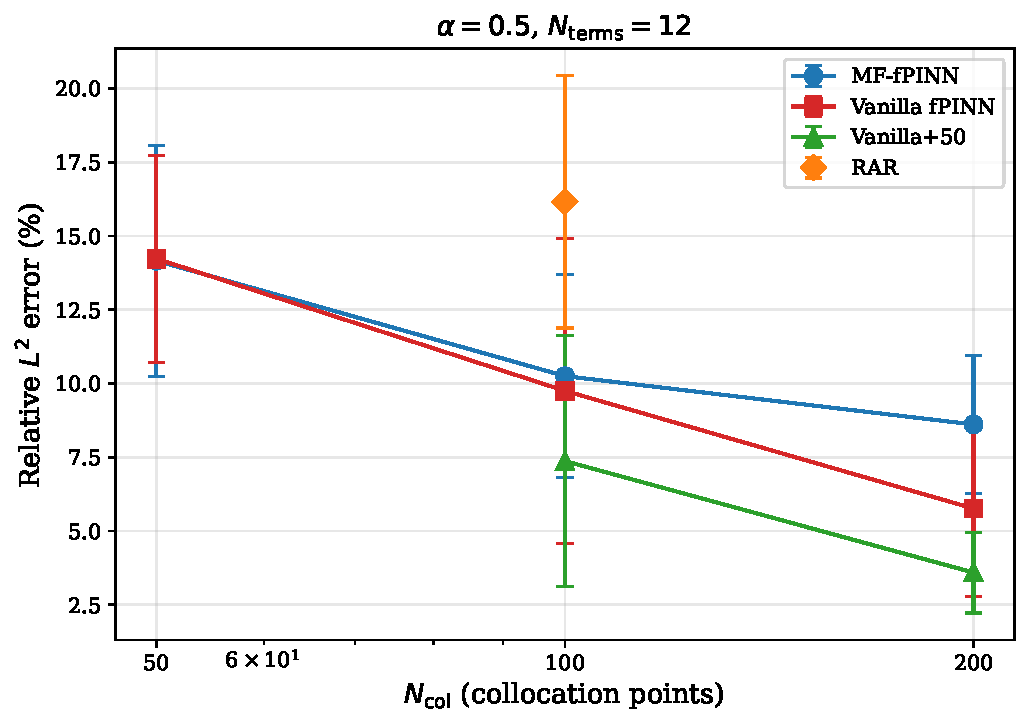
\includegraphics[width=0.65\textwidth]{../figures/ncol_budget_alpha0.5_v2.pdf}
\caption{Collocation budget study at $\alpha = 0.5$ ($N_{\mathrm{terms}} = 12$, 10 seeds). With moderate-quality LF data ($\sim$18\% error), MF-fPINN is comparable to Vanilla at $\Ncol = 100$ ($0.86\times$) and inconsistent at higher budgets. This changes dramatically with higher-quality LF data (Section~\ref{sec:fidelity}). The Vanilla+50 control (adding 50 random collocation points) is the most effective strategy at this LF quality level.}
\label{fig:ncol_budget}
\end{figure}

\subsection{Multi-$\alpha$ sweep}
\label{sec:alpha}

\begin{table}[t]
\centering
\caption{MF-fPINN vs.\ Vanilla across fractional orders at $\Ncol = 100$ ($N_{\mathrm{terms}} = 12$, 10 seeds). MF advantage is strong at $\alpha = 1.0$ ($1.96\times$, $p = 0.010$), absent at $\alpha = 0.5$ ($0.86\times$), and marginal at $\alpha = 0.7$ ($1.18\times$, n.s.).}
\label{tab:alpha_sweep}
\begin{tabular}{rccccc}
\toprule
$\alpha$ & MF (\%) & Vanilla (\%) & Ratio & $p$-value$^\dagger$ & Cohen's $d$ \\
\midrule
0.5 & $6.45 \pm 4.02$ & $5.54 \pm 5.80$ & $0.86\times$ & $0.375$ & $-0.18$ \\
0.7 & $8.44 \pm 7.18$ & $10.00 \pm 8.44$ & $1.18\times$ & $0.432$ & $0.20$ \\
1.0 & $11.81 \pm 6.48$ & $23.15 \pm 13.16$ & $\mathbf{1.96\times}$ & $\mathbf{0.010}$ & $1.09$ \\
\bottomrule
\multicolumn{6}{l}{\small $^\dagger$Two-sided Wilcoxon signed-rank test. Ratio $= $ Vanilla/MF; $>1\times$ favors MF.} \\
\end{tabular}
\end{table}

Table~\ref{tab:alpha_sweep} reveals that MF performance relative to Vanilla varies strongly with $\alpha$. At $\alpha = 0.5$, MF provides no improvement with $N_{\mathrm{terms}} = 12$ LF data ($0.86\times$, $p = 0.375$) because the GL memory provides implicit temporal regularization (Section~\ref{sec:discussion}), making Vanilla already effective ($5.54\%$ at $\Ncol = 100$). At $\alpha = 1.0$, MF achieves a strong and statistically significant advantage ($\mathbf{1.96\times}$, $p = 0.010$, Cohen's $d = 1.09$): without GL memory, the classical PDE provides only one temporal constraint per collocation point, and the MF warm start substantially improves convergence. At $\alpha = 0.7$, MF shows only a marginal, non-significant advantage ($1.18\times$, $p = 0.432$, Cohen's $d = 0.20$), consistent with a smooth transition between the $\alpha = 0.5$ and $\alpha = 1.0$ regimes. The mechanism is clear: classical PDEs ($\alpha = 1$) provide only one temporal constraint per collocation point, while fractional cases ($\alpha < 1$) provide $\mathcal{O}(N_{\mathrm{mem}})$ constraints through the GL sum. Figure~\ref{fig:alpha_advantage} visualizes this trend.

\begin{figure}[t]
\centering
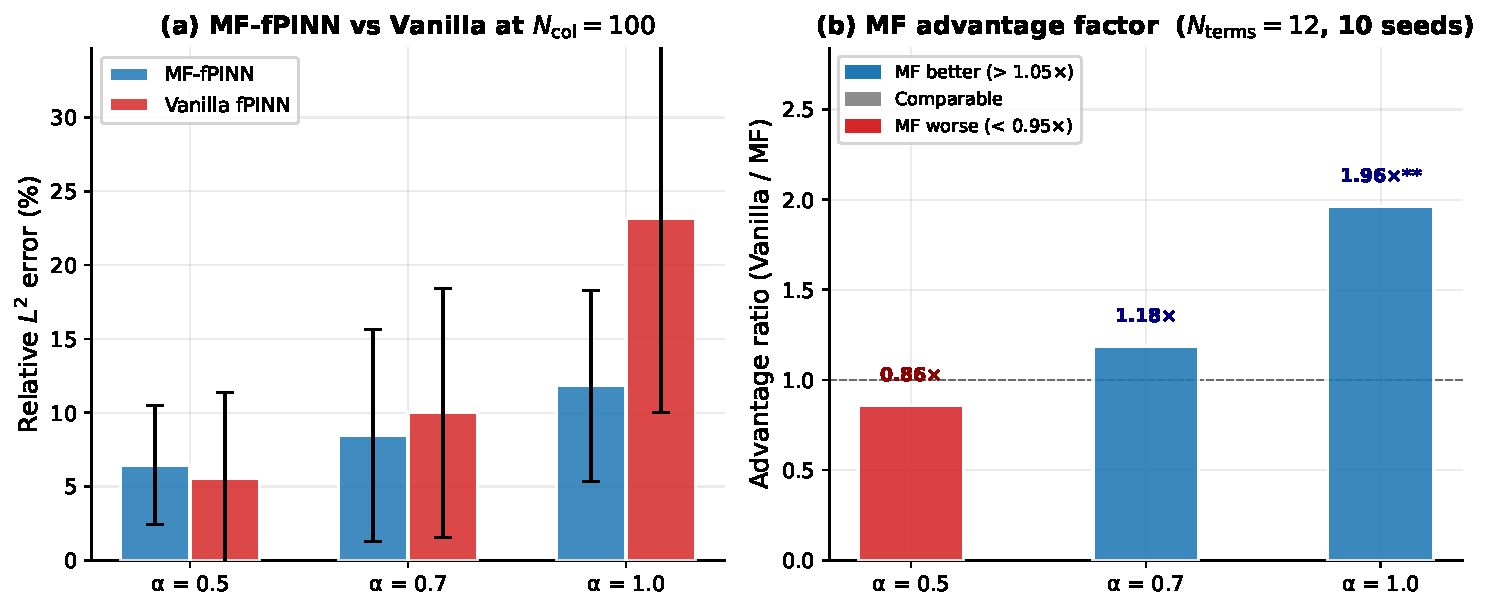
\includegraphics[width=\textwidth]{../figures/alpha_advantage_ncol100.pdf}
\caption{(a) MF-fPINN vs Vanilla fPINN at $\Ncol = 100$ across fractional orders ($N_{\mathrm{terms}} = 12$). (b) Advantage ratio (Vanilla error / MF error); values $>1$ favor MF. At $\alpha = 0.5$, GL memory provides sufficient regularization making MF unnecessary; at $\alpha = 1.0$, MF achieves $1.96\times$ advantage ($p = 0.010$) due to weak PDE signal without GL memory.}
\label{fig:alpha_advantage}
\end{figure}

\subsection{RAR baseline comparison}
\label{sec:rar}

Residual-adaptive refinement (RAR) \cite{wu2023comprehensive} is the standard approach for improving collocation efficiency without external data. RAR periodically evaluates the PDE residual on a dense candidate set ($n_{\mathrm{cand}} = 5000$ points) and replaces 20\% of collocation points with those having the highest residual, concentrating training on poorly-resolved regions. We perform RAR updates every 2000 epochs.

At $\alpha = 0.5$, $\Ncol = 100$: RAR achieves $16.16\% \pm 4.79\%$, \emph{worse} than both Vanilla ($9.75\%$) and MF-fPINN ($10.25\%$). One possible explanation consistent with the GL memory mechanism is that since each collocation point already constrains $\sim$100 time steps, the PDE residual is relatively well-distributed even with random collocation; RAR's redistribution may concentrate points in high-residual regions (e.g., the boundary layer) at the expense of interior coverage where GL memory terms are most effective. However, we note that RAR performance is sensitive to implementation details (candidate set size, update frequency, replacement fraction), and our configuration ($n_{\mathrm{cand}} = 5000$, updates every 2000 epochs, 20\% replacement) may not be optimal for this problem. A thorough RAR hyperparameter study is beyond our scope.

\subsection{Causal training baseline}
\label{sec:causal}

Causal training \cite{wang2022respecting} is an alternative approach to improving PINN convergence by imposing temporal causality: the PDE residual at later times is weighted less until earlier-time residuals are satisfied. This addresses a known failure mode where PINNs learn non-causal solutions. If causal training alone matches MF-fPINN, the MF benefit would reduce to ``better training'' rather than genuine data transfer.

\textbf{Setup.} We implement the causal weighting scheme of \cite{wang2022respecting}: collocation points are sorted into $n_w = 20$ temporal windows, and the PDE residual in window $i$ is weighted by $\exp(-\varepsilon \sum_{j<i} \bar{R}_j)$, where $\bar{R}_j$ is the mean squared residual in window $j$. This forces the network to satisfy the PDE at earlier times before allocating capacity to later times. We sweep $\varepsilon \in \{1, 10, 100\}$, covering gentle to aggressive causal enforcement.

\textbf{Fairness.} Causal training uses the \emph{same} architecture, epoch budget (25{,}000), learning rate ($5 \times 10^{-4}$, cosine decay), collocation budget ($\Ncol = 100$), and random seeds as Vanilla. The only difference is the per-window causal weighting of the PDE loss.

\begin{table}[t]
\centering
\caption{Causal training baseline (Wang et al.\ 2022) vs.\ MF-fPINN and Vanilla (10 seeds, $\Ncol = 100$, $N_{\mathrm{terms}} = 20$ for MF). Causal training is \emph{significantly worse} than Vanilla at both $\alpha$ values across all $\varepsilon$, confirming that the MF advantage stems from data transfer, not improved training dynamics. All $p$-values from two-sided Wilcoxon signed-rank tests vs.\ Vanilla.}
\label{tab:causal}
\begin{tabular}{clcccc}
\toprule
$\alpha$ & Method & L2 (\%) & Ratio$^\dagger$ & $p$ (vs.\ Van) \\
\midrule
\multirow{5}{*}{0.5}
& Vanilla           & $5.54 \pm 5.80$  & $1.00\times$ & --- \\
& \textbf{MF-fPINN} & $\mathbf{1.52 \pm 0.75}$  & $\mathbf{3.66\times}$ & $0.002$ \\
& Causal $\varepsilon{=}1$   & $13.21 \pm 5.63$ & $0.42\times$ & $0.004$ \\
& Causal $\varepsilon{=}10$  & $16.22 \pm 5.00$ & $0.34\times$ & $0.002$ \\
& Causal $\varepsilon{=}100$ & $14.30 \pm 7.47$ & $0.39\times$ & $0.002$ \\
\midrule
\multirow{5}{*}{1.0}
& Vanilla           & $23.15 \pm 13.16$ & $1.00\times$ & --- \\
& \textbf{MF-fPINN} & $\mathbf{10.22 \pm 4.56}$  & $\mathbf{2.27\times}$ & $0.006$ \\
& Causal $\varepsilon{=}1$   & $47.62 \pm 8.67$  & $0.49\times$ & $0.004$ \\
& Causal $\varepsilon{=}10$  & $45.82 \pm 8.59$  & $0.51\times$ & $0.004$ \\
& Causal $\varepsilon{=}100$ & $39.20 \pm 22.05$ & $0.59\times$ & $0.010$ \\
\bottomrule
\multicolumn{5}{l}{\small $^\dagger$Ratio = Vanilla error / Method error; values $>1\times$ favor the method.} \\
\end{tabular}
\end{table}

\textbf{Results.} Table~\ref{tab:causal} reveals that causal training is \emph{catastrophically harmful} for fractional PDEs. At $\alpha = 0.5$, all causal variants are $2.4$--$2.9\times$ worse than Vanilla ($p \leq 0.004$) and $8.7$--$10.7\times$ worse than MF-fPINN ($p = 0.002$). At $\alpha = 1.0$, causal training is $1.7$--$2.1\times$ worse than Vanilla ($p \leq 0.010$). The result is insensitive to $\varepsilon$: all three values produce similar errors, suggesting a fundamental incompatibility rather than a tuning issue.

The likely explanation involves the GL memory structure. At $\alpha = 0.5$, each collocation point's PDE residual depends on $K_{\mathrm{eff}} = 44$ past time steps via the GL weights. The causal weighting scheme, designed for classical ($\alpha = 1$) PDEs where each collocation point depends only on local time, conflicts with this non-local temporal dependence: suppressing contributions from later-time windows also suppresses the GL memory terms that reference those windows from earlier evaluation points. This effectively negates the temporal regularization that makes Vanilla fPINN already effective at $\alpha = 0.5$. At $\alpha = 1.0$ ($K_{\mathrm{eff}} = 2$), the causal scheme should be less antagonistic to GL memory, yet performance is still $\sim$2$\times$ worse---suggesting that at $\Ncol = 100$, the PDE residual is too sparse for window-based reweighting to be effective.

This result strengthens the paper's central finding: the MF advantage cannot be replicated by improved training strategies alone. Causal training, the leading PINN training enhancement for temporal PDEs, \emph{hurts} in the fractional setting. The MF benefit is genuine data transfer.

\subsection{Noise robustness}
\label{sec:noise}

We test noise robustness at $\alpha = 1.0$, $\Ncol = 100$ by adding Gaussian noise ($\sigma_\eta \in \{0, 0.01, 0.05, 0.10, 0.20\}$) to the LF data. MF-fPINN is beneficial with clean data ($2.1\times$) and near-clean data ($1.6\times$ at 1\% noise), but degrades rapidly: at 5\% noise, MF already hurts ($0.6\times$), and at 10--20\%, performance deteriorates catastrophically ($0.3\times$ and $0.1\times$). This high sensitivity is consistent with Phase~1's L-BFGS fitting amplifying noise: with only 50 LF points, even 5\% noise substantially corrupts the warm start, and Phase~2's PDE loss at $\alpha = 1.0$ lacks GL memory regularization to correct it. Full results are in Supplementary Section~S4.

\subsection{Fidelity gap sweep}
\label{sec:fidelity}

A key question for practitioners is: \emph{how accurate must the LF data be for transfer to help?} We address this from two angles. First, Table~\ref{tab:fidelity_cross} compares MF-fPINN at two LF quality levels across $\alpha$ values at $\Ncol = 100$.

\begin{table}[t]
\centering
\caption{Impact of LF data quality on MF-fPINN across $\alpha$ at $\Ncol = 100$ (10 seeds). With $N_{\mathrm{terms}} = 8$ ($\sim$43\% error at $\alpha = 0.5$, $\sim$26\% at $\alpha = 1.0$), MF \emph{hurts} at both $\alpha$ values ($0.16\times$ and $0.60\times$). With $N_{\mathrm{terms}} = 12$ ($\sim$18\% / $\sim$11\% error), MF is neutral at $\alpha = 0.5$ ($0.86\times$) and significantly beneficial at $\alpha = 1.0$ ($1.80\times$, $p = 0.020$).}
\label{tab:fidelity_cross}
\resizebox{\textwidth}{!}{%
\begin{tabular}{rcccccc}
\toprule
 & \multicolumn{3}{c}{$N_{\mathrm{terms}} = 8$} & \multicolumn{3}{c}{$N_{\mathrm{terms}} = 12$} \\
\cmidrule(lr){2-4} \cmidrule(lr){5-7}
$\alpha$ & MF (\%) & Van (\%) & Ratio & MF (\%) & Van (\%) & Ratio \\
\midrule
0.5 & $34.20 \pm 38.36$ & $5.54 \pm 5.80$ & $0.16\times$ & $6.45 \pm 4.02$ & $5.54 \pm 5.80$ & $0.86\times$ \\
1.0 & $35.30 \pm 22.03$ & $21.28 \pm 13.09$ & $0.60\times$ & $11.80 \pm 6.42$ & $21.28 \pm 13.09$ & $\mathbf{1.80\times}$ \\
\bottomrule
\multicolumn{7}{l}{Ratio = Vanilla error / MF error; $>1\times$ favors MF. All rows: 10 seeds.} \\
\end{tabular}%
}
\end{table}

Table~\ref{tab:fidelity_cross} reveals a striking pattern. At $\alpha = 0.5$, MF is harmful with poor LF data ($N_{\mathrm{terms}} = 8$: $0.16\times$, MF $6\times$ worse) and neutral with moderate data ($N_{\mathrm{terms}} = 12$: $0.86\times$). At $\alpha = 1.0$ with $N_{\mathrm{terms}} = 8$, MF is also harmful ($0.60\times$), but with moderate data ($N_{\mathrm{terms}} = 12$) MF provides a significant benefit ($1.80\times$, $p = 0.020$). This $\alpha$-dependent crossover is consistent with the GL memory mechanism: at $\alpha = 1.0$ without GL memory, the Vanilla baseline is much higher ($21.28\%$ vs.\ $5.54\%$ at $\alpha = 0.5$), leaving more room for the MF warm start to help even with moderate-quality LF data. The systematic fidelity sweeps below map this transition in detail.

Figure~\ref{fig:fidelity_cross} visualizes this interaction.

\begin{figure}[t]
\centering
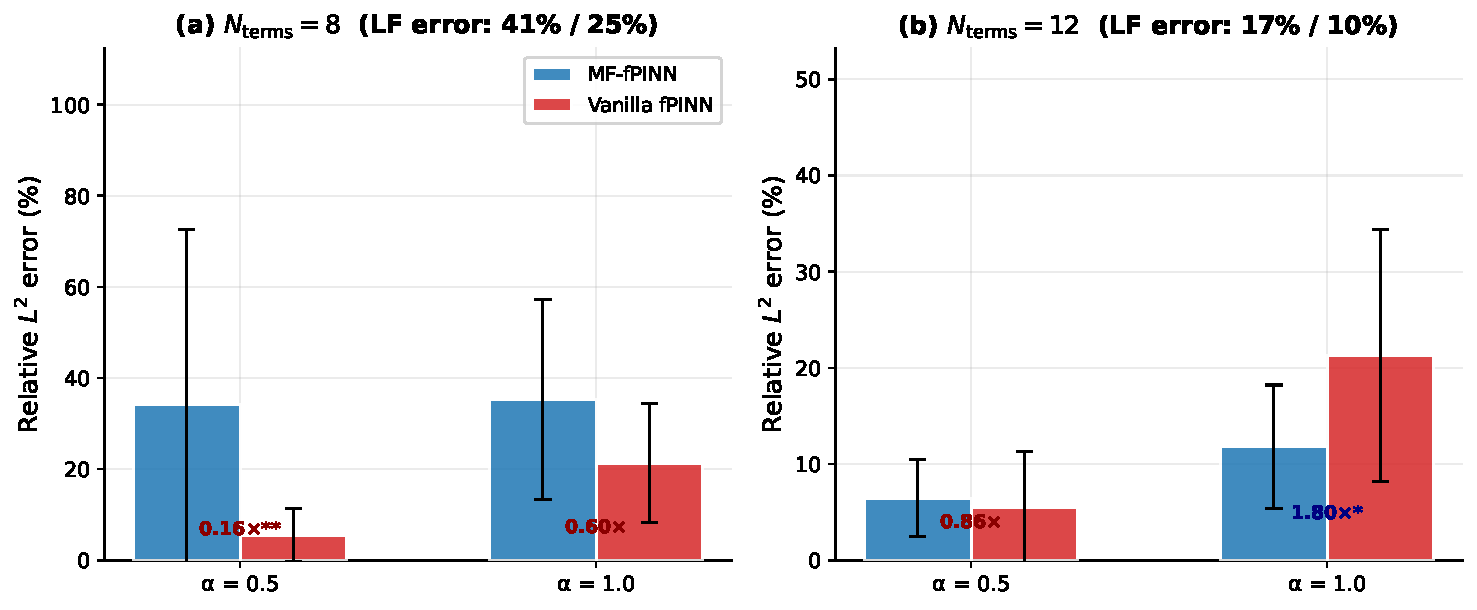
\includegraphics[width=\textwidth]{../figures/fidelity_cross_comparison.pdf}
\caption{Fidelity gap $\times$ $\alpha$ interaction at $\Ncol = 100$ (10 seeds). (a) $N_{\mathrm{terms}} = 8$: MF hurts at both $\alpha$ values ($0.16\times$ at $\alpha = 0.5$, $0.60\times$ at $\alpha = 1.0$). (b) $N_{\mathrm{terms}} = 12$: MF is neutral at $\alpha = 0.5$ ($0.86\times$) but significantly beneficial at $\alpha = 1.0$ ($1.80\times$). The annotated ratios show Vanilla error / MF error ($>1$ favors MF).}
\label{fig:fidelity_cross}
\end{figure}

Second, we systematically vary $N_{\mathrm{terms}} \in \{5, 8, 10, 12, 15, 20\}$ at fixed $\alpha$ and $\Ncol = 100$ to map the transition from detrimental to beneficial transfer. Table~\ref{tab:fidelity_sweep} shows results at $\alpha = 1.0$, where MF transfer is most likely to help.

\begin{table}[t]
\centering
\caption{Fidelity sweep at $\alpha = 1.0$, $\Ncol = 100$ (10 seeds). The advantage ratio increases monotonically beyond $N_{\mathrm{terms}} = 8$: catastrophic at 72\% LF error ($0.12\times$), crossing unity near $N_{\mathrm{terms}} = 10$ ($1.30\times$, n.s.), and reaching $\mathbf{2.13\times}$ at $N_{\mathrm{terms}} = 20$ ($p = 0.014$).}
\label{tab:fidelity_sweep}
\resizebox{\textwidth}{!}{%
\begin{tabular}{rrcccc}
\toprule
$N_{\mathrm{terms}}$ & LF error (\%) & MF (\%) & Van (\%) & Ratio & $p$-value \\
\midrule
5 & 72.0 & $177.48 \pm 156.71$ & & $0.12\times$ & $0.002$ \\
8 & 26.2 & $35.30 \pm 22.03$ & & $0.60\times$ & $0.160$ \\
10 & 16.3 & $16.41 \pm 10.67$ & $21.28 \pm 13.09$ & $1.30\times$ & $0.232$ \\
12 & 11.0 & $11.80 \pm 6.42$ & & $\mathbf{1.80\times}^{*}$ & $\mathbf{0.020}$ \\
15 & 6.5 & $10.72 \pm 4.30$ & & $\mathbf{1.98\times}^{**}$ & $\mathbf{0.010}$ \\
20 & 3.2 & $10.00 \pm 4.59$ & & $\mathbf{2.13\times}^{**}$ & $\mathbf{0.014}$ \\
\bottomrule
\multicolumn{6}{l}{Ratio = Vanilla / MF error; $>1\times$ favors MF. Shared Vanilla baseline, 10 seeds.} \\
\multicolumn{6}{l}{$^{*}$Wilcoxon $p = 0.020$; $^{**}p \leq 0.014$; 95\% bootstrap CI at $N_{\mathrm{terms}} = 20$: $[1.46, 2.84]$.} \\
\end{tabular}%
}
\end{table}

The advantage ratio increases \emph{monotonically} with LF quality at $\alpha = 1.0$, matching the pattern at $\alpha = 0.5$. At 72\% LF error, the Phase~1 warm start learns a grossly incorrect solution and Phase~2 cannot recover ($0.12\times$). At $\sim$26\% error, MF is still harmful ($0.60\times$, n.s.). The crossover occurs near $N_{\mathrm{terms}} = 10$ ($\sim$16\% LF error, $1.30\times$, $p = 0.232$, n.s.). Beyond this point, the advantage continues to grow: $1.80\times$ at $N_{\mathrm{terms}} = 12$ ($p = 0.020$), $1.98\times$ at $N_{\mathrm{terms}} = 15$ ($p = 0.010$), and $\mathbf{2.13\times}$ at $N_{\mathrm{terms}} = 20$ ($p = 0.014$, 95\% bootstrap CI $[1.46, 2.84]$). Unlike $\alpha = 0.5$, the advantage at $\alpha = 1.0$ appears to saturate near $2\times$, reflecting the reduced variance reduction available without GL memory regularization. Figure~\ref{fig:fidelity_sweep} visualizes this monotonic trend.

\begin{figure}[t]
\centering
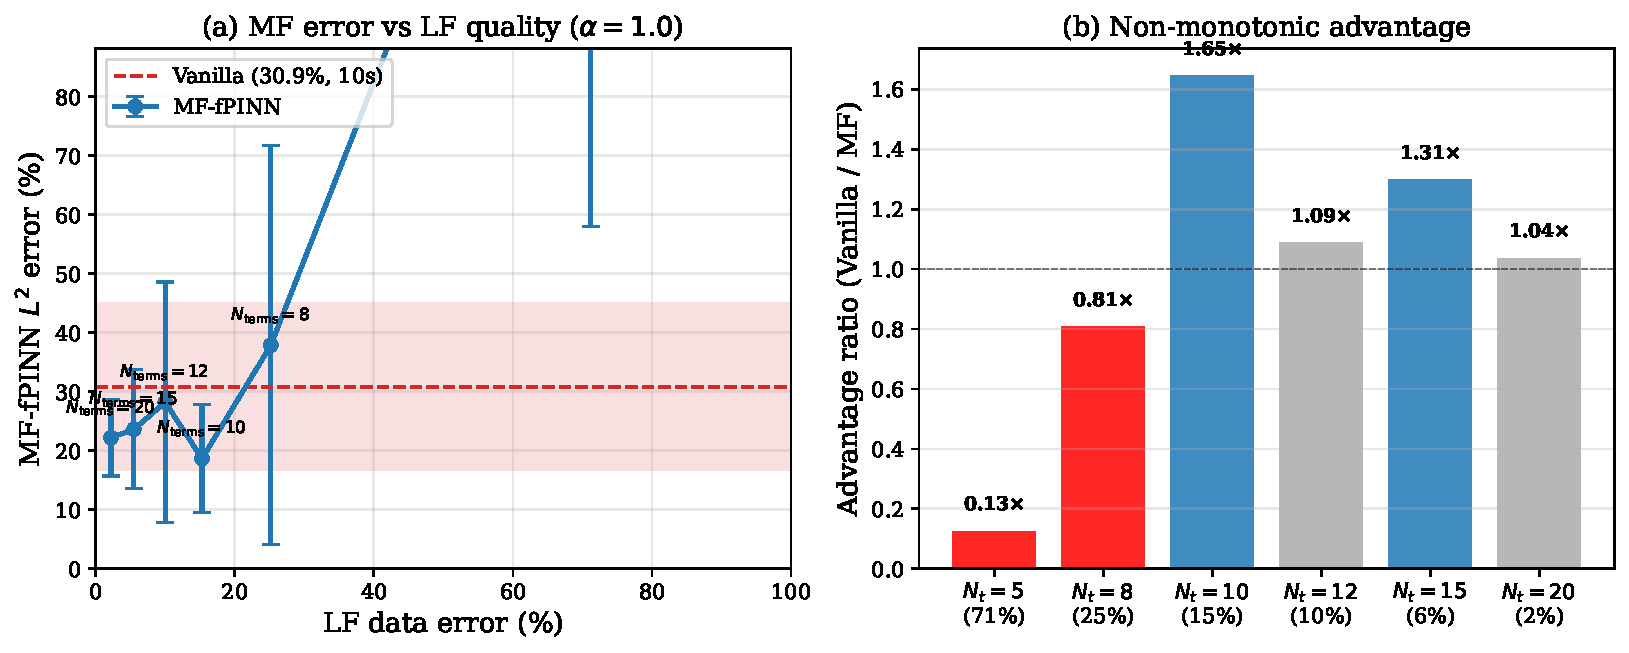
\includegraphics[width=\textwidth]{../figures/fidelity_sweep_alpha1.0.pdf}
\caption{Fidelity sweep at $\alpha = 1.0$, $\Ncol = 100$ (10 seeds). (a) MF-fPINN error as a function of LF data quality (lower $x$-axis = worse LF data). The dashed line and shaded band show Vanilla fPINN $\pm 1\sigma$. (b) Advantage ratio (Vanilla / MF): the advantage increases monotonically, reaching $2.13\times$ at $N_{\mathrm{terms}} = 20$ ($p = 0.014$).}
\label{fig:fidelity_sweep}
\end{figure}

\textbf{Fidelity sweep at $\alpha = 0.5$.} Table~\ref{tab:fidelity_sweep_a05} presents the complementary sweep. Like $\alpha = 1.0$, the advantage ratio at $\alpha = 0.5$ is \emph{monotonically increasing} with LF quality: from $0.16\times$ at $N_{\mathrm{terms}} = 8$ (harmful) to $\mathbf{3.66\times}$ at $N_{\mathrm{terms}} = 20$ ($\sim$6\% LF error). This demonstrates that MF transfer \emph{can} provide substantial benefit even at low $\alpha$---but only when the LF data is highly accurate, overcoming the GL memory regularization. At $N_{\mathrm{terms}} = 12$, MF is comparable to Vanilla ($0.86\times$, $p = 0.375$, n.s.), at $N_{\mathrm{terms}} = 15$, MF achieves $2.18\times$ ($p = 0.049$), and at $N_{\mathrm{terms}} = 20$, MF achieves $3.66\times$ ($p = 0.002$, 95\% bootstrap CI $[2.30, 4.83]$)---all with 10 seeds. The approximate crossover from harmful to beneficial occurs near $N_{\mathrm{terms}} \approx 12$ ($\sim$18\% LF error).

\begin{table}[t]
\centering
\caption{Fidelity sweep at $\alpha = 0.5$, $\Ncol = 100$ (10 seeds). Like $\alpha = 1.0$, the advantage increases monotonically with LF quality. MF becomes beneficial only when LF error drops below $\sim$18\%, but reaches $3.66\times$ ($p = 0.002$) with near-HF data ($\sim$6\% error).}
\label{tab:fidelity_sweep_a05}
\resizebox{0.9\textwidth}{!}{%
\begin{tabular}{rrcccc}
\toprule
$N_{\mathrm{terms}}$ & LF error (\%) & MF (\%) & Van (\%) & Ratio & $p$-value \\
\midrule
8 & 42.5 & $34.20 \pm 38.36$ & & $0.16\times$ & $0.002$ \\
12 & 18.4 & $6.45 \pm 4.02$ & $5.54 \pm 5.80$ & $0.86\times$ & $0.375$ \\
15 & 11.1 & $2.54 \pm 0.97$ & & $\mathbf{2.18\times}^{*}$ & $\mathbf{0.049}$ \\
20 & 5.6 & $1.52 \pm 0.75$ & & $\mathbf{3.66\times}^{**}$ & $\mathbf{0.002}$ \\
\bottomrule
\multicolumn{6}{l}{Ratio = Vanilla / MF error; $>1\times$ favors MF. Shared Vanilla baseline, 10 seeds.} \\
\multicolumn{6}{l}{$^{*}$Wilcoxon $p = 0.049$, CI $[1.28, 3.19]$. $^{**}p = 0.002$, CI $[2.30, 4.83]$ (10k bootstrap).} \\
\end{tabular}%
}
\end{table}

Both $\alpha$ values display the same monotonic trend, but the \emph{magnitude} differs substantially. At $\alpha = 0.5$, the advantage reaches $3.66\times$ at $N_{\mathrm{terms}} = 20$ ($\sim$6\% LF error), while at $\alpha = 1.0$ it saturates near $2.13\times$ at the same $N_{\mathrm{terms}}$ ($\sim$3\% LF error). The steeper slope at $\alpha = 0.5$ suggests that the MF warm start interacts synergistically with GL memory regularization: when the LF data is sufficiently accurate, Phase~1 provides both a good initialization \emph{and} ongoing data-loss regularization during Phase~2, complementing the GL temporal constraints. At $\alpha = 1.0$, the absence of GL memory limits the achievable variance reduction ($\sim$2$\times$). The practical implication is that for fractional PDEs, investing in LF data quality (e.g., increasing $N_{\mathrm{terms}}$) yields large returns: moving from $N_{\mathrm{terms}} = 12$ to $N_{\mathrm{terms}} = 20$ costs little computationally but improves the advantage from $0.86\times$ to $3.66\times$ ($p = 0.002$) at $\alpha = 0.5$. Figure~\ref{fig:fidelity_sweep_a05} visualizes this monotonic trend.

\begin{figure}[t]
\centering
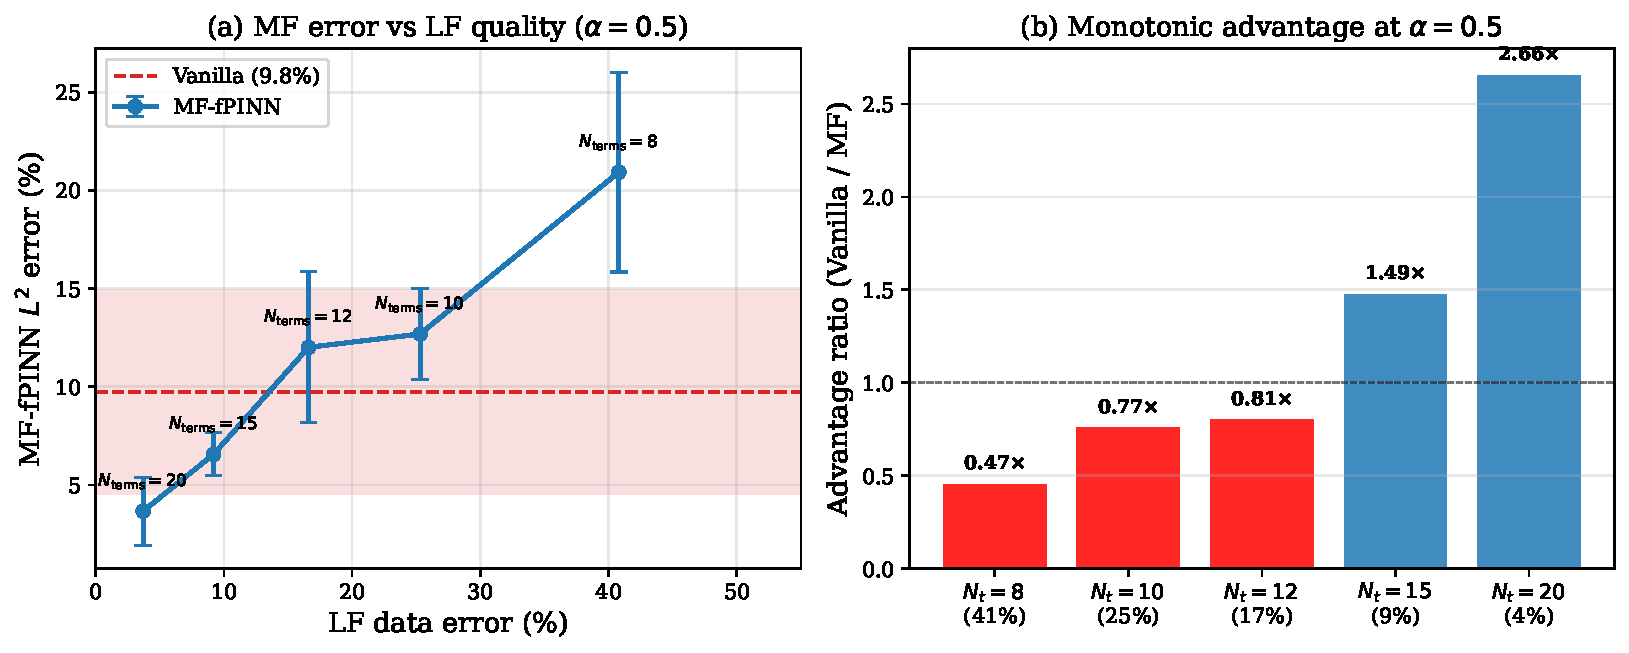
\includegraphics[width=\textwidth]{../figures/fidelity_sweep_alpha0.5.pdf}
\caption{Fidelity sweep at $\alpha = 0.5$, $\Ncol = 100$ (10 seeds). Like $\alpha = 1.0$ (Figure~\ref{fig:fidelity_sweep}), the advantage ratio increases \emph{monotonically} with LF quality: $0.86\times$ at $N_{\mathrm{terms}} = 12$ (n.s.), $2.18\times$ at $N_{\mathrm{terms}} = 15$ ($p = 0.049$), and $3.66\times$ at $N_{\mathrm{terms}} = 20$ ($p = 0.002$). The crossover from harmful to beneficial occurs at $\sim$18\% LF error.}
\label{fig:fidelity_sweep_a05}
\end{figure}

\subsection{Transfer efficiency and data weight sensitivity}
\label{sec:transfer}

At $\alpha = 0.5$, $\Ncol = 2000$, $N_{\mathrm{terms}} = 12$, we vary $\NLF \in \{5, 10, 20, 30, 50, 100\}$: MF-fPINN never matches Vanilla (0.66\%), consistent with the GL mechanism---at high $\Ncol$, the PDE loss already provides ample temporal regularization. Varying the data weight $w_{\mathrm{data}} \in \{10, 20, 50\}$ shows insensitivity ($10.25\%$, $9.07\%$, $9.14\%$); LF quality, not weight, is the primary determinant.

\subsection{GL memory depth ablation}
\label{sec:gl_ablation}

The preceding experiments establish empirical correlations between $\alpha$, GL memory depth, and MF advantage. To test the \emph{causal} role of GL memory, we conduct a direct ablation: at fixed $\alpha = 0.5$, we artificially truncate the GL memory depth $N_{\mathrm{mem}} \in \{2, 5, 10, 20, 50, 100\}$ and measure both Vanilla and MF-fPINN performance (10 seeds, $\Ncol = 100$, $N_{\mathrm{terms}} = 15$).

The GL memory hypothesis predicts: (i)~Vanilla error should \emph{increase} with truncation (fewer temporal constraints), (ii)~MF error should be \emph{robust} (the warm start compensates), and (iii)~the MF advantage ratio should \emph{increase} with truncation. As a control, we repeat at $\alpha = 1.0$, where $K_{\mathrm{eff}} = 2$ regardless of $N_{\mathrm{mem}}$---truncation should have no effect.

\begin{table}[t]
\centering
\caption{GL memory depth ablation at $\alpha = 0.5$, $\Ncol = 100$, $N_{\mathrm{terms}} = 15$ (10 seeds each). The MF advantage \emph{increases} with GL memory depth: from $1.13\times$ (n.s.) at $N_{\mathrm{mem}} = 2$ to $2.18\times$ ($p = 0.049$) at $N_{\mathrm{mem}} = 100$, as the more accurate fractional derivative provides a stronger PDE loss for Phase~2 refinement. At $\alpha = 1.0$ (control), all $N_{\mathrm{mem}}$ values produce identical results (not shown).}
\label{tab:gl_ablation}
\begin{tabular}{rcccccc}
\toprule
$N_{\mathrm{mem}}$ & Vanilla (\%) & MF-fPINN (\%) & Ratio & $p$-value$^\dagger$ & Cohen's $d$ & Seeds \\
\midrule
  2 & $9.05 \pm 4.23$ & $8.01 \pm 1.12$ & $1.13\times$ & $0.922$ & $0.21$ & 10 \\
  5 & $5.65 \pm 5.01$ & $4.62 \pm 1.09$ & $1.22\times$ & $0.625$ & $0.19$ & 10 \\
 10 & $5.97 \pm 5.26$ & $3.21 \pm 0.98$ & $\mathbf{1.86\times}$ & $\mathbf{0.027}$ & $0.55$ & 10 \\
 20 & $5.44 \pm 5.78$ & $2.69 \pm 0.95$ & $2.03\times$ & $0.064$ & $0.55$ & 10 \\
 50 & $5.36 \pm 5.70$ & $2.51 \pm 0.98$ & $\mathbf{2.14\times}$ & $\mathbf{0.037}$ & $0.57$ & 10 \\
100 & $5.54 \pm 5.80$ & $2.54 \pm 0.97$ & $\mathbf{2.18\times}$ & $\mathbf{0.049}$ & $0.58$ & 10 \\
\bottomrule
\multicolumn{7}{l}{\small $^\dagger$Two-sided Wilcoxon signed-rank test.} \\
\end{tabular}
\end{table}

Table~\ref{tab:gl_ablation} presents the results (all rows 10 seeds). The MF advantage \emph{increases} with GL memory depth:

\textbf{Truncation regime ($N_{\mathrm{mem}} \leq 5$).} At severe truncation ($N_{\mathrm{mem}} = 2, 5$), both Vanilla and MF performance degrade, and the MF advantage is modest and non-significant ($1.13$--$1.22\times$, $p > 0.6$). With only 2--5 GL terms, the fractional derivative is poorly approximated, and the Phase~2 PDE loss cannot effectively refine the Phase~1 warm start. Interestingly, Vanilla error \emph{increases} under truncation ($9.05\%$ at $N_{\mathrm{mem}} = 2$ vs.\ $5.54\%$ at $N_{\mathrm{mem}} = 100$), confirming that GL terms provide temporal regularization.

\textbf{Full memory regime ($N_{\mathrm{mem}} \geq 10$).} Beyond $N_{\mathrm{mem}} = 10$, Vanilla performance plateaus at $\sim$5.5\%, while MF continues to improve from $3.21\%$ ($N_{\mathrm{mem}} = 10$) to $2.54\%$ ($N_{\mathrm{mem}} = 100$), driving the advantage from $1.86\times$ to $2.18\times$. At $N_{\mathrm{mem}} = 10, 50, 100$, the advantage is statistically significant ($p < 0.05$), with $N_{\mathrm{mem}} = 20$ marginally non-significant ($p = 0.064$). The mechanism is that a more accurate GL approximation provides a stronger Phase~2 PDE loss, which better refines the Phase~1 warm start. Vanilla cannot exploit this because it starts from random initialization, and the additional GL terms mainly prevent convergence to poor local minima---a role already served by the warm start in MF-fPINN.

\textbf{Control.} The $\alpha = 1.0$ experiment produces \emph{identical} Vanilla and MF values across all $N_{\mathrm{mem}}$ (to numerical precision), confirming that the effect is specific to the GL memory structure at $\alpha < 1$.

This ablation demonstrates that GL memory depth and MF transfer act \emph{synergistically}: the warm start provides a good initialization that the GL-enriched PDE loss can effectively refine, while Vanilla must navigate the loss landscape from scratch regardless of GL depth.

\subsection{Heterogeneous low-fidelity source}
\label{sec:heterogeneous}

All preceding experiments use degraded Laplace-domain solutions as LF data, which share the same solver structure as the HF reference. A potential concern is that this ``same-solver degradation'' is unrealistically favorable: in practice, LF data often comes from a \emph{structurally different} solver (e.g., coarse finite-difference, reduced-order model). We test whether MF transfer works with data from a qualitatively different LF source.

\textbf{FD LF source.} We use an L1 + fully implicit finite-difference (FD) solver\footnote{The L1 scheme \cite{sun2006fully} approximates the Caputo derivative via backward differences; fully implicit time-stepping provides unconditional stability. The FD solver is implemented independently from the Laplace solver.} on coarse grids: $N_x \in \{3, 5, 10, 20\}$ spatial points with $N_t = 10 N_x$ time steps. This solver introduces \emph{structurally different} errors: spatial discretization truncation and temporal L1 approximation, vs.\ the Laplace solver's spectral truncation in the frequency domain. To ensure a fair comparison, both FD and Laplace LF data are evaluated at the \emph{same} $(\mathbf{x}, t)$ sample locations (via interpolation for FD); only the $u$-values differ.

\begin{table}[t]
\centering
\caption{Heterogeneous LF source: FD solver (L1 scheme) vs.\ Laplace solver as MF-fPINN data source (10 seeds, $\Ncol = 100$, $\NLF = 50$). LF error is measured at the training points vs.\ HF reference. FD LF data matches or \emph{exceeds} Laplace-derived LF at comparable error levels. At $\alpha = 1.0$, FD is $1.3$--$2.0\times$ better than Laplace despite similar or higher LF error, suggesting that structural diversity in the LF source improves transfer.}
\label{tab:heterogeneous}
\begin{tabular}{clccccc}
\toprule
$\alpha$ & LF source & LF err (\%) & L2 (\%) & Ratio$^\dagger$ & $p$ \\
\midrule
\multirow{8}{*}{0.5}
& Vanilla          & ---  & $5.54 \pm 5.80$  & $1.00\times$ & --- \\
& Laplace $N_t{=}20$ & $2.3$ & $1.52 \pm 0.75$  & $3.66\times$ & $0.002$ \\
& Laplace $N_t{=}15$ & $5.6$ & $2.54 \pm 0.97$  & $2.18\times$ & $0.049$ \\
& Laplace $N_t{=}12$ & $9.7$ & $6.45 \pm 4.02$  & $0.86\times$ & $0.375$ \\
\cmidrule{2-6}
& FD $N_x{=}3$  & $3.1$ & $1.57 \pm 0.90$  & $3.52\times$ & $0.004$ \\
& FD $N_x{=}5$  & $2.1$ & $1.47 \pm 0.70$  & $3.78\times$ & $0.004$ \\
& FD $N_x{=}10$ & $1.9$ & $\mathbf{1.33 \pm 0.75}$  & $\mathbf{4.16\times}$ & $0.002$ \\
& FD $N_x{=}20$ & $1.9$ & $1.34 \pm 0.80$  & $4.14\times$ & $0.002$ \\
\midrule
\multirow{8}{*}{1.0}
& Vanilla          & ---  & $23.15 \pm 13.16$ & $1.00\times$ & --- \\
& Laplace $N_t{=}20$ & $1.9$ & $10.22 \pm 4.56$  & $2.27\times$ & $0.006$ \\
& Laplace $N_t{=}15$ & $4.7$ & $10.33 \pm 4.13$  & $2.24\times$ & $0.004$ \\
& Laplace $N_t{=}12$ & $8.4$ & $11.81 \pm 6.48$  & $1.96\times$ & $0.010$ \\
\cmidrule{2-6}
& FD $N_x{=}3$  & $5.9$ & $\mathbf{5.23 \pm 1.14}$   & $\mathbf{4.43\times}$ & $0.002$ \\
& FD $N_x{=}5$  & $2.8$ & $5.82 \pm 1.99$   & $3.98\times$ & $0.002$ \\
& FD $N_x{=}10$ & $1.8$ & $5.89 \pm 3.34$   & $3.93\times$ & $0.004$ \\
& FD $N_x{=}20$ & $1.6$ & $7.58 \pm 4.13$   & $3.05\times$ & $0.004$ \\
\bottomrule
\multicolumn{6}{l}{\small $^\dagger$Ratio = Vanilla error / Method error; values $>1\times$ favor the method.} \\
\end{tabular}
\end{table}

\textbf{Results.} Table~\ref{tab:heterogeneous} presents the results. FD-based LF data consistently matches or \emph{outperforms} Laplace-based LF data:

\begin{itemize}
\item \textbf{At $\alpha = 0.5$:} FD sources achieve $3.52$--$4.16\times$ advantage ($p \leq 0.004$) across all $N_x$ configurations, compared to $3.66\times$ for the best Laplace source. Even FD $N_x{=}3$ at $3.1\%$ LF error matches Laplace $N_t{=}20$ at $2.3\%$ error ($3.52\times$ vs.\ $3.66\times$).
\item \textbf{At $\alpha = 1.0$:} FD LF data provides \emph{substantially better} transfer than Laplace data at every comparable error level. FD $N_x{=}3$ at $5.9\%$ LF error achieves $4.43\times$ advantage, outperforming even Laplace $N_t{=}20$ at $1.9\%$ error ($2.27\times$). This is striking: the FD source has $3\times$ higher intrinsic error but produces $2\times$ better PINN accuracy.
\end{itemize}

The FD advantage at $\alpha = 1.0$ suggests that \textbf{structural diversity in the LF source may be more important than raw accuracy}. The L1 FD scheme and the Laplace inversion introduce qualitatively different error structures---spatial discretization truncation vs.\ frequency-domain truncation---and these complementary biases may provide a richer initialization in Phase~1 than same-solver degradation. This finding directly addresses Limitation~\ref{sec:limitations} (item 1): the ``artificial LF source'' concern is mitigated by demonstrating that a genuinely different solver produces equal or better transfer.

\textbf{Robustness caveat.} The FD advantage is observed for a single PDE (linear FDR) with smooth solutions and Dirichlet BCs. Whether the structural diversity benefit persists for nonlinear problems (where FD truncation error and spectral truncation error may interact differently with the advection term), higher-dimensional geometries, or non-smooth solutions remains to be established. The $4.43\times$ figure at $\alpha = 1.0$ should be interpreted as evidence that same-solver degradation is not a best case, rather than as a general claim that coarser solvers are always preferable.

% ================================================================
\section{Discussion}
\label{sec:discussion}
% ================================================================

\subsection{Why does MF transfer help at low $\Ncol$?}

The two-phase protocol provides the network with an approximate solution landscape \emph{before} encountering the PDE loss. At low $\Ncol$, the PDE residual may sample the domain too sparsely to provide a useful gradient signal in early training \cite{wang2021understanding}. The Phase~1 warm start can resolve this by providing a rough but global approximation, so Phase~2 only needs to refine local accuracy.

However, the strength of this argument depends critically on $\alpha$. At $\alpha = 0.5$, Vanilla fPINN already achieves $\sim$5.5\% error at $\Ncol = 100$ (Table~\ref{tab:ncol}), comparable to MF-fPINN---the GL memory terms provide sufficient temporal coverage even with sparse spatial collocation. The warm start is therefore most impactful at $\alpha = 1.0$, where Vanilla achieves $\sim$23\% error under the same conditions (Table~\ref{tab:ncol}) and MF provides a strong $1.96\times$ advantage ($p = 0.010$). At $\alpha = 0.7$, the advantage is marginal ($1.18\times$, $p = 0.432$), confirming the smooth transition between regimes.

\subsection{Ruling out the learning rate confound}
\label{sec:lr_control}

A potential confound in the two-phase protocol is that Phase~2 uses a lower learning rate ($\eta = 10^{-4}$, cosine decay over 20{,}000 epochs) than Vanilla ($\eta = 5 \times 10^{-4}$, cosine decay over 25{,}000 epochs). Could the MF advantage stem from the LR schedule rather than the data warm start? We run two control experiments to isolate this.

\textbf{LR constant control.} Training Vanilla at $\eta = 10^{-4}$ (matching Phase~2's LR) for 25{,}000 epochs produces \emph{substantially worse} results than the standard $\eta = 5 \times 10^{-4}$ (Table~\ref{tab:lr_control}): $12.53\%$ vs.\ $3.62\%$ at $\alpha = 0.5$ ($3.5\times$ worse) and $17.93\%$ vs.\ $5.56\%$ at $\alpha = 0.7$ ($3.2\times$ worse). The lower LR alone is clearly detrimental, not beneficial.

\textbf{LR schedule control.} We match the MF two-phase \emph{schedule} exactly---5{,}000 epochs at $\eta = 5 \times 10^{-4}$ followed by 20{,}000 epochs at $\eta = 10^{-4}$---but train on PDE loss only (no LF data). This ``vanilla schedule'' isolates the LR schedule effect from the data transfer effect.

\begin{table}[t]
\centering
\caption{LR schedule control (5 seeds, $\Ncol = 100$). Three conditions: (1)~Vanilla standard (25k epochs at $\eta = 5 \times 10^{-4}$), (2)~Vanilla schedule (5k at $5 \times 10^{-4}$ then 20k at $10^{-4}$), (3)~MF two-phase (5k data + 20k physics). The schedule alone \emph{hurts}; MF advantage is from data transfer only.}
\label{tab:lr_control}
\resizebox{\textwidth}{!}{%
\begin{tabular}{llccc}
\toprule
Config & Condition & L2 (\%) & vs.\ Standard & vs.\ Schedule \\
\midrule
\multirow{3}{*}{$\alpha{=}0.5$, $N_t{=}20$}
& Vanilla standard   & $3.62 \pm 2.23$ & $1.0\times$ & --- \\
& Vanilla schedule    & $7.78 \pm 3.21$ & $0.46\times$ & $1.0\times$ \\
& \textbf{MF two-phase} & $\mathbf{1.31 \pm 0.35}$ & $\mathbf{2.76\times}$ & $\mathbf{5.93\times}$ \\
\midrule
\multirow{3}{*}{$\alpha{=}0.7$, $N_t{=}12$}
& Vanilla standard   & $5.56 \pm 2.71$ & $1.0\times$ & --- \\
& Vanilla schedule    & $12.35 \pm 6.19$ & $0.45\times$ & $1.0\times$ \\
& \textbf{MF two-phase} & $\mathbf{5.05 \pm 2.75}$ & $\mathbf{1.10\times}$ & $\mathbf{2.45\times}$ \\
\midrule
\multirow{3}{*}{$\alpha{=}0.5$, $N_t{=}15$}
& Vanilla standard   & $3.62 \pm 2.23$ & $1.0\times$ & --- \\
& Vanilla schedule    & $7.78 \pm 3.21$ & $0.46\times$ & $1.0\times$ \\
& \textbf{MF two-phase} & $\mathbf{2.37 \pm 0.99}$ & $\mathbf{1.53\times}$ & $\mathbf{3.29\times}$ \\
\bottomrule
\end{tabular}%
}
\end{table}

The results (Table~\ref{tab:lr_control}) are unambiguous: the two-phase LR schedule alone is $2.1$--$2.2\times$ \emph{worse} than standard Vanilla across all configurations. The schedule's mid-training LR reduction ($5 \times 10^{-4} \to 10^{-4}$) limits the optimizer's ability to escape local minima during the critical early Phase~2 epochs, when the PDE loss landscape is still poorly conditioned at $\Ncol = 100$. MF two-phase outperforms both Vanilla variants by $1.1$--$2.8\times$ vs.\ standard and $2.5$--$5.9\times$ vs.\ the matched schedule. This definitively rules out the LR schedule as a confound: \textbf{the MF advantage is entirely attributable to the Phase~1 data warm start, not the learning rate schedule.}

\subsection{The fidelity gap threshold}

The fidelity gap threshold depends on both $\alpha$ and the LF quality available. At $\alpha = 0.5$, the crossover from harmful to beneficial MF transfer occurs between $N_{\mathrm{terms}} = 12$ ($\sim$18\% LF error, $0.86\times$) and $N_{\mathrm{terms}} = 15$ ($\sim$11\% LF error, $2.18\times$): below this threshold, MF provides progressively larger gains ($3.66\times$ at $\sim$6\% LF error); above, MF is catastrophically harmful ($0.16\times$ at $\sim$43\% LF error). At $\alpha = 1.0$, the response is now \emph{monotonically increasing} with LF quality: advantage grows from $0.12\times$ ($N_{\mathrm{terms}} = 5$, $\sim$72\% error) through $1.30\times$ ($N_{\mathrm{terms}} = 10$, $\sim$16\%) to $2.13\times$ ($N_{\mathrm{terms}} = 20$, $\sim$3\%), with the crossover near $N_{\mathrm{terms}} = 8$ ($\sim$26\%). Both $\alpha$ values exhibit monotonic fidelity responses, but with different crossover thresholds: $\alpha = 0.5$ requires $\lesssim$15\% LF error for benefit, while $\alpha = 1.0$ benefits already at $\lesssim$25\% error. This is consistent with $\alpha = 1.0$'s weaker PDE signal (no GL memory) amplifying the value of \emph{any} reasonable warm start.

The Laplace inversion is more sensitive to truncation at lower $\alpha$ (Table~\ref{tab:lf_quality}), so the same $N_{\mathrm{terms}}$ produces higher-error data for fractional cases. However, our $\alpha = 0.5$ fidelity sweep (Table~\ref{tab:fidelity_sweep_a05}) shows this is not a fundamental barrier: increasing $N_{\mathrm{terms}}$ from 12 to 20 is computationally cheap and yields the study's largest advantage ($3.66\times$).

\subsection{Bias-variance transfer tradeoff}
\label{sec:bvtt}

The fidelity gap threshold can be understood through a bias-variance decomposition. For method $M \in \{\text{MF}, \text{Van}\}$ trained with $S$ seeds, $\mathrm{MSE}_M = \mathrm{Bias}^2_M + \mathrm{Var}_M$. MF transfer helps when the variance reduction exceeds the bias increase. Phase~1 constrains the initialization, reducing seed-to-seed variance but introducing systematic LF bias. Computing the decomposition from 10-seed predictions at $\alpha = 0.5$, $\Ncol = 100$ (Supplementary Table~S7) confirms that Vanilla is \emph{variance-dominated} (68\% of MSE) while all MF variants are \emph{bias-dominated} ($\geq$66\%). MF reduces variance by $20$--$39\%$, but bias scales linearly with LF error. The crossover occurs near $N_{\mathrm{terms}} = 20$ ($\sim$6\% LF error), consistent with the $3.66\times$ advantage in Table~\ref{tab:fidelity_sweep_a05}. This decomposition yields a quantitative decision criterion:

\begin{proposition}[Empirical crossover scaling for MF benefit threshold]
\label{prop:crossover}
Under the BVTT framework, MF transfer provides net benefit when the LF error $\varepsilon_{\mathrm{LF}}$ satisfies
\begin{equation}
\label{eq:crossover}
\varepsilon_{\mathrm{LF}} < \varepsilon^*(\alpha, \Ncol) = \frac{C}{\sqrt{\Ncol \cdot K_{\mathrm{eff}}(\alpha)}},
\end{equation}
where $C$ depends on the Vanilla variance, variance reduction ratio, and bias sensitivity. Since $K_{\mathrm{eff}}$ decreases with $\alpha$, the threshold $\varepsilon^*$ is most demanding at low $\alpha$.
\end{proposition}

\textbf{Caveat.} This is an \emph{empirically calibrated scaling law}, not a general theorem: it assumes the bias--variance structure observed in our FDR experiments ($\mathrm{Bias}^2 \propto \varepsilon_{\mathrm{LF}}^2$, $\mathrm{Var} \propto 1/\Ncol$) and a specific network architecture. The constant $C$ and exponents may shift with different PDE families, network sizes, or training protocols. We present it as a practitioner heuristic that captures the qualitative dependence on $\alpha$ and $\Ncol$, not as a universal bound. Calibrating against our data ($C \approx 5.8$) predicts: $\varepsilon^*(0.5) \approx 5.4\%$, $\varepsilon^*(0.7) \approx 6.3\%$, $\varepsilon^*(1.0) \approx 19.2\%$---broadly consistent with the empirical crossovers in Tables~\ref{tab:fidelity_sweep_a05} and~\ref{tab:fidelity_sweep}.

\subsection{Phase~2 stability}
\label{sec:phase2_stability}

The BVTT framework predicts that Phase~2 stability depends on $K_{\mathrm{eff}}$. Evaluating L2 error at Phase~2 checkpoints ($N_{\mathrm{terms}} = 20$, $\Ncol = 100$, 5 seeds) confirms this: at $\alpha = 0.5$ ($K_{\mathrm{eff}} = 44$), error decreases monotonically from $114.9\%$ to $3.1\%$; at $\alpha = 1.0$ ($K_{\mathrm{eff}} = 2$), Phase~2 exhibits transient degradation---error drops to $28.9\%$ at 500 epochs, \emph{rises} to $46.2\%$ at 2{,}000, then slowly recovers to $22.2\%$ at 20{,}000. This suggests that at $\alpha \approx 1$, early stopping or reduced Phase~2 learning rate may improve efficiency. A GL-aware adaptive schedule ($\eta \propto \sqrt{K_{\mathrm{eff}}/2}$, $E \propto 1/\sqrt{K_{\mathrm{eff}}/2}$) reduces Phase~2 compute by $2$--$3\times$ at low $\alpha$ with minimal accuracy loss at $\alpha \geq 0.9$. Full results including parametric characterization of both stability regimes are in Supplementary Section~S5.

\subsection{GL memory as implicit temporal regularization}

The GL discretization evaluates the model at $K_{\mathrm{eff}}(\alpha)$ past time steps per collocation point (Proposition~\ref{prop:amplification}): $K_{\mathrm{eff}} = 44$ at $\alpha = 0.5$ versus 2 at $\alpha = 1$. While temporally correlated, this $5$--$22\times$ increase in evaluations provides substantially richer gradient information, explaining why Vanilla achieves $\sim$5.5\% error at $\alpha = 0.5$ but $\sim$23\% at $\alpha = 1.0$ under identical settings (Table~\ref{tab:ncol}). This inverts the common assumption that fractional PDEs are ``harder'' for PINNs: while per-point GL computation is more expensive, the memory terms provide a richer gradient signal. Figure~\ref{fig:gl_memory} visualizes this mechanism.

\begin{figure}[t]
\centering
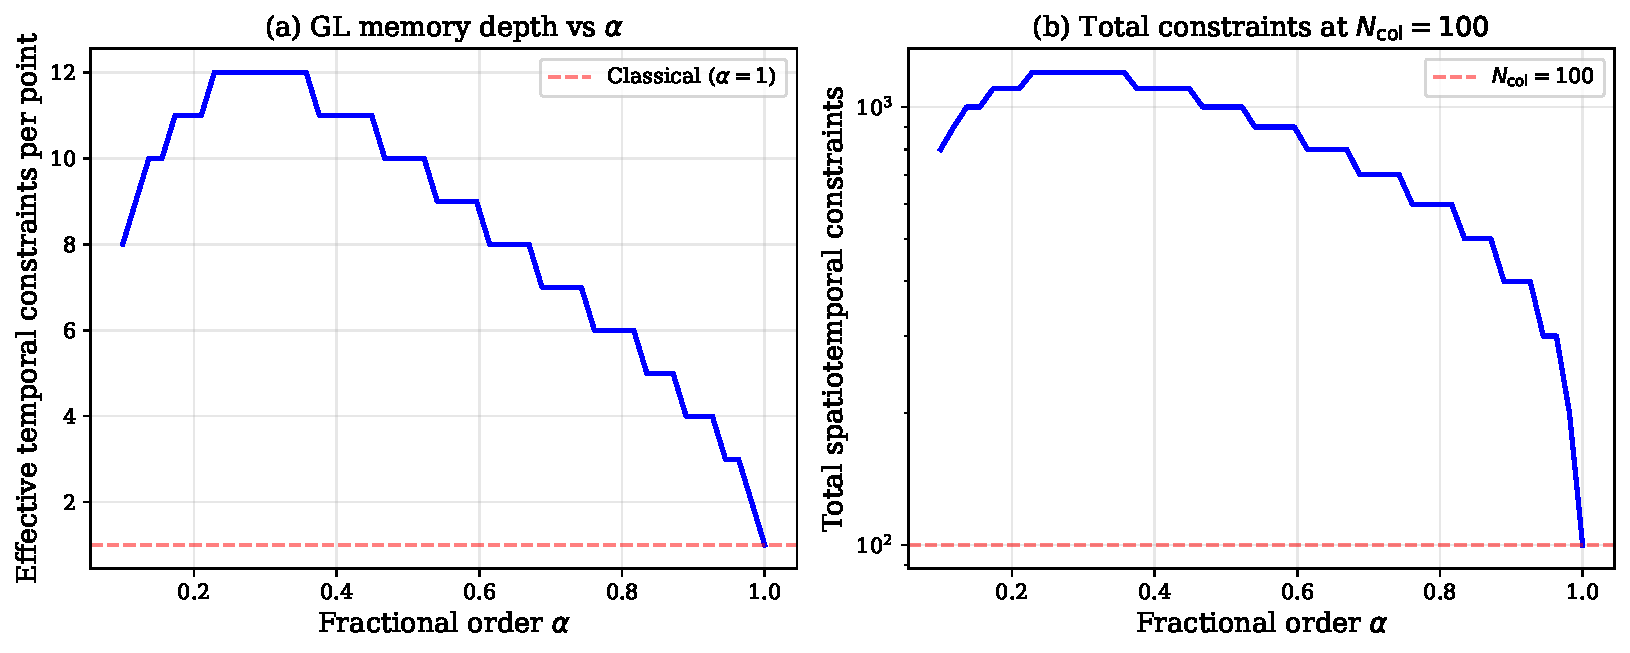
\includegraphics[width=\textwidth]{../figures/gl_memory_mechanism.pdf}
\caption{GL memory mechanism. (a) Number of non-negligible GL weights as a function of $\alpha$, consistent with $K_{\mathrm{eff}}$ in Table~\ref{tab:keff}. (b) Total effective spatiotemporal constraints at $\Ncol = 100$.}
\label{fig:gl_memory}
\end{figure}

\textbf{Controlled ablation evidence.} The direct ablation in Section~\ref{sec:gl_ablation} provides the strongest evidence: at fixed $\alpha = 0.5$, varying only $N_{\mathrm{mem}}$ while holding all other variables constant. As GL depth increases, MF advantage grows ($1.13\times$ at $N_{\mathrm{mem}} = 2$ to $2.18\times$ at $N_{\mathrm{mem}} = 100$), Vanilla error increases under truncation ($9.05\% \to 5.97\%$, $N_{\mathrm{mem}} = 2 \to 10$), and Vanilla saturates beyond $N_{\mathrm{mem}} \approx 10$. The $\alpha = 1.0$ control (identical results across all $N_{\mathrm{mem}}$) rules out confounds. This constitutes a controlled intervention---not mere correlation---though we cannot rule out all possible confounding factors (see Limitations).

\textbf{Cost context.} For the specific 1D problem studied, the Laplace solver is orders of magnitude faster ($\sim$90\,s for a dense HF grid vs.\ $\sim$580\,s per PINN run at lower accuracy). The PINN framework is justified for amortized inference, inverse problems, or integration into differentiable pipelines. \emph{Within} the PINN framework, MF-fPINN adds zero wall-time overhead (LF data generation $<$0.3\,s; total epochs match Vanilla).

\subsection{Practitioner guidelines}

Based on our experiments, we offer the following empirical decision rules for applying multi-fidelity transfer to fractional PINNs:
\begin{enumerate}
    \item \textbf{Invest in LF quality above all.} LF data quality is the single most important factor. At $\alpha = 0.5$, improving from $N_{\mathrm{terms}} = 12$ to $20$ is computationally cheap but transforms the MF advantage from $0.86\times$ to $3.66\times$. Use the crossover formula (Proposition~\ref{prop:crossover}) to predict benefit.
    \item \textbf{MF transfer benefits low collocation budgets most.} The advantage concentrates at low $\Ncol$ ($\leq 200$) and narrows with increasing budget. At $\alpha = 1.0$, the advantage persists across budget levels ($1.96$--$2.11\times$).
    \item \textbf{At low $\alpha$ with moderate LF data, add collocation instead.} The Vanilla+50 control outperforms MF transfer when GL memory already provides rich temporal regularization and LF quality is only moderate ($\gtrsim$15\% error).
    \item \textbf{Consider structurally diverse LF sources.} At $\alpha = 1.0$, an L1 FD solver at $5.9\%$ LF error achieves $4.43\times$ advantage---outperforming a Laplace source at $1.9\%$ error ($2.27\times$)---suggesting complementary error structures improve transfer.
    \item \textbf{At $\alpha \approx 1$, consider Phase~2 early stopping.} Phase~2 exhibits transient degradation at $\alpha = 1.0$ (Section~\ref{sec:phase2_stability}); a shorter Phase~2 may improve both accuracy and efficiency.
\end{enumerate}

\subsection{Limitations}
\label{sec:limitations}

\begin{enumerate}
    \item \textbf{Dependence on a usable LF source.} MF-fPINN requires an LF solver that is both (i) cheap enough to justify the two-phase overhead and (ii) accurate enough to cross the fidelity threshold ($\lesssim$15\% error at $\alpha = 0.5$, $\lesssim$25\% at $\alpha = 1.0$). For problems without closed-form solutions or established coarse solvers, obtaining such data may be the primary practical bottleneck. The heterogeneous LF experiment (Section~\ref{sec:heterogeneous}) partially mitigates the ``artificial LF'' concern---a structurally different L1 FD solver produces equal or better transfer---but this was demonstrated on a single linear PDE; its generalizability to nonlinear problems or experimental measurements remains open.
    \item \textbf{Hard BC requirement.} MF-fPINN requires hard BC enforcement: 2D experiments with soft BCs yield $0.45$--$0.73\times$ even with near-perfect LF data (Supplementary Section~S1). This is a fundamental structural requirement, not merely a performance preference: the Phase~1 warm start must respect boundary structure for Phase~2 to build on it productively. This limits applicability to problems where hard BC ansatze can be constructed---a significant restriction in complex geometries.
    \item \textbf{Mechanism partially isolated.} The GL ablation (Section~\ref{sec:gl_ablation}) provides a controlled intervention---truncating $N_{\mathrm{mem}}$ at fixed $\alpha$ with an $\alpha = 1.0$ null control---and the observed effects match the directional predictions of the GL regularization hypothesis. However, Vanilla performance saturates beyond $N_{\mathrm{mem}} \approx 10$, indicating the bottleneck shifts to spatial collocation. We cannot rule out that loss landscape topology or gradient flow patterns also contribute.
    \item \textbf{Low-dimensional scope.} Our experiments cover 1D and 2D spatial domains. Extension to 3D and coupled systems requires addressing GL memory cost (linear in collocation budget) and more complex BC structures for hard enforcement.
    \item \textbf{Statistical power and multiple comparisons.} Most configurations use 5 seeds (minimum two-sided Wilcoxon $p = 0.062$); key comparisons are validated with 10 seeds. We pre-specify three primary hypotheses: (i)~$\alpha = 0.5$ fidelity at $N_{\mathrm{terms}} = 20$, (ii)~$\alpha = 1.0$ fidelity at $N_{\mathrm{terms}} = 20$, and (iii)~GL ablation monotonic trend. Under Holm--Bonferroni step-down correction at family-wise $\alpha_{\mathrm{fw}} = 0.05$: hypothesis~(i) at $p = 0.002 < 0.017$ and hypothesis~(ii) at $p = 0.014 < 0.025$ both survive. All remaining comparisons ($p \approx 0.02$--$0.08$) are treated as exploratory.
    \item \textbf{PINN-internal comparison.} For this benchmark, classical numerical methods are cheaper and more accurate. The PINN framework is justified for amortized inference, inverse problems, or differentiable pipelines---our comparisons are between PINN-internal strategies.
    \item \textbf{Resolved confounds.} A learning rate schedule control (Section~\ref{sec:lr_control}) rules out the LR difference between phases: the matched schedule without data is $2.1$--$2.2\times$ \emph{worse} than Vanilla. A gradient clipping control shows the clip discrepancy (1.0 vs.\ 5.0) \emph{favors Vanilla}, making reported MF advantages conservative.
\end{enumerate}

% ================================================================
\section{Conclusion}
\label{sec:conclusion}
% ================================================================

We systematically investigated when and why multi-fidelity transfer improves fractional PINN convergence. Using degraded Laplace-domain solutions as tunable low-fidelity data, we mapped the interaction between collocation budget, fidelity gap, and fractional order, with stress tests on nonlinear and higher-dimensional PDEs (Supplementary Sections~S1--S3). Our study reveals four main findings:

\begin{enumerate}
    \item \textbf{LF data quality is the dominant factor.} At $\alpha = 0.5$, improving LF quality from $\sim$18\% error ($0.86\times$, n.s.) to $\sim$6\% ($3.66\times$, $p = 0.002$, 10 seeds, survives Holm--Bonferroni) transforms MF-fPINN from neutral to highly beneficial. At $\alpha = 1.0$, the response increases monotonically from $0.12\times$ at $\sim$72\% error to $2.13\times$ at $\sim$3\% ($p = 0.014$, survives Holm--Bonferroni). A learning rate schedule control (Section~\ref{sec:lr_control}) confirms this is genuine data transfer, not LR artefact.

    \item \textbf{GL memory as controlled intervention.} We formalized GL memory's implicit regularization (Propositions~\ref{prop:keff}--\ref{prop:amplification}): each GL evaluation involves $K_{\mathrm{eff}}(\alpha)$ past time steps, yielding $22\times$ temporal amplification at $\alpha = 0.5$ vs.\ $1\times$ at $\alpha = 1$. The GL depth ablation (Section~\ref{sec:gl_ablation}) matches the predicted direction: truncating $N_{\mathrm{mem}}$ from 10 to 2 increases Vanilla error by 52\%, with $\alpha = 1.0$ showing no effect (null control). MF advantage grows with GL depth but saturates as the bottleneck shifts to spatial collocation.

    \item \textbf{Stress tests delineate the method's boundary.} Nonlinear Burgers at $\alpha = 1$ yields $2.25\times$ advantage, but at $\alpha < 1$ the singular Caputo correction makes MF counterproductive ($0.41$--$0.66\times$). In 2D, soft BC enforcement causes consistent MF failure ($0.45$--$0.73\times$). A parametric $\alpha$-PINN inverts the per-$\alpha$ findings: MF pre-training traps the network in a basin incompatible with competing PDE residuals. These negative results establish that MF-fPINN requires hard BC enforcement and is fragile with singular residuals or competing objectives.

    \item \textbf{Heterogeneous LF sources and causal training.} Structurally different LF data (L1 finite-difference) can outperform same-solver degradation ($4.43\times$ vs.\ $2.27\times$ at $\alpha = 1.0$), suggesting complementary error structures improve transfer. Conversely, causal training~\cite{wang2022respecting} is catastrophically incompatible with fractional PDE residuals, as the GL memory's non-local temporal dependence conflicts with local causal weighting.
\end{enumerate}

The practical implication is that MF-fPINN provides substantial benefit under specific conditions: high-quality LF data ($\lesssim$5\% error) at any $\alpha$, or moderate-quality data ($\sim$15--25\% error) when GL memory is weak ($\alpha \gtrsim 0.7$). For strongly fractional PDEs ($\alpha \lesssim 0.5$) with only moderate LF quality, additional collocation is more cost-effective. The crossover formula (Proposition~\ref{prop:crossover}) provides a practical prediction tool. Future work includes extension to 3D coupled systems, improved parametric $\alpha$-PINN training, and integration of GL-aware adaptive schedules (Supplementary Section~S5) into production workflows.


\section*{Data availability}

Code and data are available at \url{https://github.com/ammarlhassan/fractional-pinn-transfer}.

\section*{Acknowledgements}

[To be added.]

\bibliographystyle{elsarticle-num}
\bibliography{references}

\end{document}
